\documentclass[conference]{IEEEtran}
\IEEEoverridecommandlockouts

\usepackage{cite}
\usepackage{amsmath,amssymb,amsfonts}
\usepackage{graphicx}
\graphicspath{{figures/}{./}}
\usepackage{textcomp}
\usepackage{booktabs}
\usepackage{array}
\usepackage{url}
\usepackage{multirow}
\usepackage{xcolor}

\begin{document}

\title{Eco Life Buddy: An AI-Based CCTV Monitoring System for Detecting Public Cleanliness and Waste Disposal Violations}

\author{

\IEEEauthorblockN{
\begin{tabular}{ccc}
 Balaji R & Saravanan S & Vigneshayyanar M \\
Dept. of M.Tech. CSE & Dept. of M.Tech. CSE & Dept. of M.Tech. CSE \\
Sri Sairam Engineering College & Sri Sairam Engineering College & Sri Sairam Engineering College \\
Chennai, India & Chennai, India & Chennai, India \\
balajiraviseetha@gmail.com & saravanan1442005@gmail.com & vigneshayyanar134@gmail.com
\end{tabular}
}

\vspace{0.35cm}

\IEEEauthorblockN{
\begin{tabular}{c}
Dr. M. Nithya\\
Dept. of M.Tech. CSE \\
Sri Sairam Engineering College \\
Chennai, India \\
nithya.m@sairam.edu.in
\end{tabular}
}

}

\maketitle

%%------------------------------------------------------------
\begin{abstract}
Maintaining cleanliness in shared urban environments is an escalating operational challenge for municipal authorities, institutions, and civic bodies. Conventional Closed-Circuit Television (CCTV) infrastructure operates primarily as passive recording hardware, necessitating continuous manual supervision that is labor-intensive, error-prone, and slow to respond. This paper presents Eco Life Buddy, an autonomous AI-powered CCTV surveillance framework designed to detect public cleanliness violations and improper waste disposal in real time. The system employs YOLO26 as its core detection backbone, capitalizing on its end-to-end Non-Maximum Suppression (NMS)-free architecture, dual-label assignment head, Progressive Loss (ProgLoss) formulation, and optimized edge-computing throughput. Object detections are coupled with ByteTrack-augmented multi-object tracking, spatial-temporal proximity analysis, and an interpretable rule-based decision engine to reliably classify complex events including active littering, waste abandonment, and improper bin disposal. The system suppresses common urban confusers (e.g., vendors setting down goods, resting luggage, sanitation worker collections), archives tamper-evident encrypted evidence frames, and dispatches multi-channel alerts to enforcement personnel. 

Experimental evaluation on a real-world CCTV benchmark across five urban environments in Chennai, India, demonstrates superior detection accuracy, achieving a mean Average Precision at IoU 0.50 ($\text{mAP}_{50}$) of 93.0\% and $\text{mAP}_{50\text{-}95}$ of 70.9\%. At the event level across 184 test clips, the system achieves an overall F1-score of 0.892 (95\% CI: [0.841, 0.930]) with a false alarm rate of 4.9\%. In continuous 72-hour evaluations on unedited CCTV footage under realistic low base rates, the system generates only 2.8 false alarms per camera-day with an average detection delay of 1.38 seconds. The raw detector achieves 322.6 frames per second (FPS) on an NVIDIA RTX 3090, while the full end-to-end analytics pipeline sustains 32.4 FPS per camera stream, exceeding standard 30 FPS video rates. The framework incorporates human-in-the-loop verification, audit logs compliant with India's Digital Personal Data Protection (DPDP) Act 2023, and spatial kernel density estimation for municipal resource optimization.
\end{abstract}

\begin{IEEEkeywords}
Artificial Intelligence, Smart Surveillance, YOLO26, Multi-Object Tracking, Public Cleanliness, Littering Detection, Temporal Event Analysis, Spatial Reasoning, Smart Cities, Edge Computing.
\end{IEEEkeywords}

%%------------------------------------------------------------
\section{Introduction}
\label{sec:intro}

Rapid urbanization has intensified the operational complexity of managing public hygiene and municipal solid waste in modern metropolitan areas. Unlawful behaviors such as roadside dumping, casual littering, and improper waste placement incur severe repercussions for public health, stormwater drainage maintenance, urban aesthetics, and environmental sustainability \cite{b1}. The United Nations Environment Programme (UNEP) estimates that over 2.1 billion tonnes of municipal solid waste are generated globally every year, with outdoor public disposal violations accounting for a significant portion of unmanaged municipal waste \cite{b2}. Municipalities lacking continuous automated monitoring mechanisms face escalating cleanup expenditures and deteriorating civic compliance.

Although contemporary smart cities have deployed dense grids of fixed IP surveillance cameras across public transit hubs, market corridors, parks, and residential neighborhoods, the vast majority of these systems remain passive recording devices. Routine monitoring relies upon human operators observing banks of video monitors or conducting retrospective reviews after citizen grievances are lodged. Human visual inspection degrades substantially over prolonged surveillance shifts due to cognitive fatigue, inattention, and multi-feed divided focus \cite{b11}. Consequently, violations go largely undetected at the moment of occurrence, eliminating deterrence and weakening civic accountability.

Recent breakthroughs in deep learning and real-time computer vision offer a transformative opportunity to convert passive CCTV infrastructure into active, automated compliance monitoring systems \cite{b4, b12}. Modern single-stage object detectors can detect visual targets in cluttered scenes with sub-5-millisecond latency. Furthermore, coupling high-speed detectors with spatial-temporal association models enables the interpretation of multi-frame human-object interactions without requiring computationally prohibitive 3D video classification backbones. From an urban governance perspective, continuous visual analytics also unlocks aggregate spatial intelligence: by aggregating detected violation coordinates over time, municipal authorities can synthesize spatial density heatmaps to identify recurring littering hotspots, optimize bin placement, and schedule targeted sanitation patrols \cite{b13}.

This paper introduces \textit{Eco Life Buddy}, a complete, real-time AI-based CCTV surveillance framework tailored specifically for public cleanliness monitoring. At the core of the proposed system is the integration of the latest YOLO26 detection backbone \cite{b3}. Released in January 2026 by Ultralytics, YOLO26 provides crucial architectural advancements for edge surveillance: natively end-to-end inference via dual-label assignment that completely eliminates post-processing Non-Maximum Suppression (NMS), removal of the Distribution Focal Loss (DFL) module for hardware-agnostic edge compilation, fine-tuning stabilization using the MuSGD optimizer, and Progressive Loss (ProgLoss) for multi-scale feature alignment \cite{b3}.

Beyond raw object detection, this work addresses the scientific challenge of distinguishing genuine civic violations from ambiguous everyday interactions. Prior surveillance systems often suffer from high false positive rates caused by benign confusers, such as vendors resting merchandise crates, commuters resting luggage, or municipal sweepers collecting litter. Eco Life Buddy resolves these ambiguities through a multi-stage reasoning pipeline that couples ByteTrack multi-object tracking, spatial proximity modeling, dynamic region-of-interest (ROI) zone compliance, and an interpretable rule-based decision engine with inverse-action filtering.

The primary contributions of this paper are summarized as follows:
\begin{itemize}
\item \textbf{End-to-End Surveillance Framework:} A multi-camera CCTV analytics pipeline combining fine-tuned YOLO26 object detection with spatial-temporal event reasoning to autonomously detect active littering, waste abandonment, and improper bin disposal.
\item \textbf{NMS-Free Real-Time Backbone:} Deployment of YOLO26 with MuSGD optimization and ProgLoss multi-scale bounding box regression, delivering raw inference throughput of 322.6 FPS on GPU (3.1 ms latency) and sustaining full end-to-end pipeline processing at 32.4 FPS per camera stream.
\item \textbf{Spatial-Temporal Event Engine:} A trajectory-aware reasoning module incorporating person-waste proximity gating ($d_{pw}$), disposal zone compliance ($d_{wb}$), minimum observation windows ($\tau_{\min}$), and cooldown throttling ($\tau_{cd}$) to prevent transient false alarms.
\item \textbf{Urban Confuser and Sanitation Worker Filtering:} Formal operational definitions and suppression logic co-designed with municipal stakeholders to filter everyday non-violations (resting bags, street vendor goods, wind-blown debris) and distinguish compliant municipal sweepers via inverse-action tracking.
\item \textbf{Continuous Long-Duration Validation:} Comprehensive empirical validation including a clip-level benchmark (184 test clips, 0.892 F1-score with 95\% confidence intervals) and a continuous 72-hour unedited deployment evaluation demonstrating a low false alarm rate of 2.8 alarms per camera-day.
\item \textbf{Ethical and DPDP-Compliant Infrastructure:} Complete evidence management with tamper-evident encrypted archiving (AES-256), automated redaction, human-in-the-loop review workflow, appeals audit mechanisms compliant with India's DPDP Act 2023, and municipal GIS heatmap aggregation for sanitation planning.
\end{itemize}

The rest of this paper is structured as follows: Section~\ref{sec:related} reviews relevant literature. Section~\ref{sec:problem} formalizes the problem statement and operational violation criteria. Section~\ref{sec:method} presents the proposed methodology and architectural components. Section~\ref{sec:arch} details the seven-layer system architecture. Section~\ref{sec:dataset} details dataset collection, annotation protocols, ethics approvals, and implementation parameters. Section~\ref{sec:eval} reports experimental evaluations, continuous deployment results, sensitivity analyses, and baseline comparisons. Section~\ref{sec:discuss} discusses deployment governance, DPDP compliance, and limitations. Finally, Section~\ref{sec:conc} concludes the paper.

%%------------------------------------------------------------
\section{Related Work}
\label{sec:related}

\subsection{Object Detection in Waste and Litter Surveillance}

Early visual surveillance systems relied predominantly on classical background subtraction algorithms (e.g., Gaussian Mixture Models) and handcrafted spatial descriptors such as Histograms of Oriented Gradients (HOG) and Scale-Invariant Feature Transform (SIFT) \cite{b14}. However, these approaches exhibited severe sensitivity to dynamic lighting variations, moving shadows, wind-induced background motion, and cluttered urban textures.

The advent of deep convolutional neural networks revolutionized visual monitoring. Single-stage detectors from the YOLO family \cite{b4, b5} and SSD \cite{b6} reframed detection as a direct spatial bounding box regression task, achieving real-time inference rates. In environmental surveillance, researchers applied YOLO architectures to roadside garbage detection and municipal sorting. Nayfeh et al.\ \cite{b7} demonstrated a two-stage YOLOv8 pipeline for classifying 16 urban waste categories, reporting an mAP of 88.9\%. Automated street waste detection systems such as Street-YOLO \cite{b8} achieved 90.6\% mAP on curated road imagery. Large-scale public benchmarks such as the TACO (Trash Annotations in Context) dataset \cite{b21} provided standardized annotations for litter objects in outdoor contexts, driving further advancements in small-object litter detection. Beyond single-stage CNN detectors, transformer-based architectures such as DETR have demonstrated competitive accuracy for fine-grained object detection, but their high computational complexity hampers real-time edge execution \cite{b15}.

Despite these advancements, standard detectors historically depended on Non-Maximum Suppression (NMS) as a post-processing heuristic. NMS incurs unpredictable, input-dependent execution overhead on embedded hardware and frequently suppresses valid overlapping targets in crowded surveillance scenes. YOLO26 overcomes this structural bottleneck through end-to-end dual-label assignment, producing one-to-one predictions directly during inference without NMS \cite{b3}, rendering it exceptionally suitable for continuous CCTV monitoring.

\subsection{Temporal Modeling and Action Recognition}

Detecting an isolated waste item in a single video frame is fundamentally insufficient to ascertain whether a civic violation occurred. A beverage container on the pavement may have been dropped moments earlier by a passing pedestrian, abandoned hours prior, or blown into the scene by wind. Discriminating deliberate littering from incidental presence demands temporal reasoning over consecutive frames.

Two primary paradigms exist for video-based event interpretation: learned spatio-temporal video classification backbones and trajectory-based tracking engines. Dense video classification architectures, such as CNN-LSTM hybrids \cite{b9}, MoViNet \cite{b10}, and X3D \cite{b23}, capture complex temporal dynamics across multi-frame video clips. Similarly, dense optical flow estimators \cite{b16} and skeleton-based graph convolutional networks \cite{b17} model fine-grained motion patterns. Alharbi et al.\ \cite{b10} applied MoViNet to identify vehicular and pedestrian littering actions, achieving 93.7\% classification accuracy. However, dense 3D video classification networks exhibit two critical drawbacks for edge surveillance: first, they require buffering multi-second clips (imposing a 2-to-5 second latency penalty before inference can even commence); second, their high computational and memory footprint severely restricts concurrent processing across multi-camera streams.

Conversely, tracking-based reasoning extracts lightweight object and person trajectories and applies spatial-temporal state machines to evaluate event rules. This paradigm operates with zero buffering delay, requires minimal computational overhead, and provides full decision interpretability for municipal authorities.

\subsection{Multi-Object Tracking in Surveillance}

Multi-Object Tracking (MOT) links detected bounding boxes into consistent trajectories across frames. SORT popularized the combination of the Kalman filter for motion forecasting and the Hungarian algorithm for data association \cite{b18}. DeepSORT augmented this formulation with deep appearance re-identification (ReID) embeddings to maintain identities across occlusions \cite{b19}. More recently, ByteTrack demonstrated that associating low-confidence detection boxes—rather than discarding them outright—significantly improves tracking continuity in crowded or occluded scenes while maintaining high processing speeds \cite{b22}. The proposed framework leverages ByteTrack-enhanced association, ensuring robust tracking of both small waste items and pedestrians across momentary visual occlusions.

\subsection{Integrated Cleanliness Surveillance Platforms}

Several integrated surveillance prototypes have been reported in the smart city literature. Park et al.\ \cite{b20} introduced a campus CCTV anomaly detection framework combining background subtraction and CNN classifiers to identify debris accumulation. However, their system operated on isolated frames without temporal behavior modeling, resulting in elevated false positive rates in dynamic environments. 

Crucially, existing literature lacks an end-to-end framework that unifies an NMS-free detection backbone (YOLO26), trajectory-based event gating, dynamic disposal zone polygon reasoning, municipal confuser filtering, and continuous long-recording operational verification within a single deployable architecture. Eco Life Buddy directly addresses this gap.

%%------------------------------------------------------------
\section{Problem Definition and Operational Criteria}
\label{sec:problem}

\subsection{Mathematical Problem Formulation}

Consider a continuous video stream $\mathcal{V} = \{f_1, f_2, \ldots, f_T\}$ captured by a fixed surveillance camera at a nominal frame rate of $R$ frames per second (FPS). The objective of the surveillance system is to detect the occurrence of a public cleanliness violation event $E$ at timestamp $t$ and generate a cryptographically verifiable evidence package for municipal review.

Formally, a violation event $E$ is defined as a tuple:
\begin{equation}
E = \langle P_k,\; O_m,\; \mathcal{Z},\; \Delta t,\; \Theta \rangle
\end{equation}
where $P_k$ denotes the tracked bounding box trajectory of person $k$, $O_m$ denotes the trajectory of waste item $m$, $\mathcal{Z}$ represents the designated compliant disposal zone (defined as an ROI polygon or proximity radius around an authorized bin), $\Delta t$ represents the observation observation window, and $\Theta = \{\theta_{det}, \theta_{conf}\}$ denotes the detection and event confirmation confidence thresholds.

The spatial Euclidean distance $d(P_k, O_m)$ between person centroid $(x_{P}, y_{P})$ and waste item centroid $(x_{O}, y_{O})$ at frame $t$ is expressed as:
\begin{equation}
d(P_k, O_m) = \sqrt{(x_{P} - x_{O})^2 + (y_{P} - y_{O})^2}
\end{equation}

To ensure robustness against camera tilt angles and distance perspective distortion, we introduce perspective-normalized distance scaling. Given the bounding box height $h_{P}$ of the associated person, the normalized spatial distance $\tilde{d}(P_k, O_m)$ is computed as:
\begin{equation}
\tilde{d}(P_k, O_m) = \frac{d(P_k, O_m)}{h_{P} / \bar{h}_{ref}}
\end{equation}
where $\bar{h}_{ref}$ is a reference human height constant (calibrated to 160 pixels at nominal ground distance). The person-waste proximity condition is satisfied when:
\begin{equation}
\tilde{d}(P_k, O_m) \leq d_{pw}
\end{equation}
where $d_{pw}$ is the configured proximity threshold (default $d_{pw} = 120$ px).

Similarly, the waste-to-bin proximity condition evaluates whether the waste centroid $(x_O, y_O)$ lies within compliant disposal zone polygon $\mathcal{Z}$ or satisfies:
\begin{equation}
d(O_m, B_j) = \sqrt{(x_O - x_{B_j})^2 + (y_O - y_{B_j})^2} \leq d_{wb}
\end{equation}
where $B_j$ is the centroid of nearest detected bin $j$ and $d_{wb}$ is the acceptable disposal tolerance radius (default $d_{wb} = 80$ px).

\subsection{Operational Violation Definitions}

In coordination with municipal solid waste management stakeholders, three distinct violation classes and two compliant non-violation classes are formally defined:

\begin{enumerate}
\item \textbf{Active Littering ($V_1$):} A person trajectory $P_k$ is observed carrying or co-located with a waste item $O_m$ ($\tilde{d} \leq d_{pw}$), followed by the physical separation of $O_m$ such that $O_m$ becomes stationary outside any compliant disposal zone $\mathcal{Z}$ ($\tilde{d}(O_m, B) > d_{wb}$), while $P_k$'s trajectory diverges ($\tilde{d}(P_k, O_m) > d_{pw}$) and persists for $\Delta t \geq \tau_{\min}$.
\item \textbf{Waste Abandonment ($V_2$):} A stationary waste object $O_m$ persists outside any authorized disposal zone $\mathcal{Z}$ for a prolonged duration $\tau_{ab} \geq 450$ frames (15 seconds at 30 FPS) without any associated person track within proximity $d_{pw}$.
\item \textbf{Improper Bin Disposal ($V_3$):} A person $P_k$ deposits waste $O_m$ in the immediate vicinity of an authorized bin $B_j$ ($d(O_m, B_j) \leq 2 \times d_{wb}$), but outside the designated bin aperture or polygon boundary ($O_m \notin \mathcal{Z}$), indicating careless placement or overflow negligence.
\item \textbf{Compliant Disposal ($C_1$):} Waste item $O_m$ is deposited strictly within the designated ROI polygon $\mathcal{Z}$ or inside bin boundary $B_j$ ($d(O_m, B_j) \leq d_{wb}$), triggering violation suppression.
\item \textbf{Background Activity ($C_2$):} Normal pedestrian transit, vehicular traffic, or static environmental objects with no active or stationary waste interaction.
\end{enumerate}

\subsection{Handling Everyday Municipal Confusers}

A major vulnerability of simplistic proximity-rule systems is the generation of spurious alarms in response to benign daily activities. To prevent alert fatigue among municipal enforcement staff, Eco Life Buddy implements specific suppression filters for four common urban confusers:

\begin{itemize}
\item \textbf{Resting Luggage / Bags:} Commuters frequently place backpacks, shopping bags, or briefcases on the pavement while waiting. To prevent misclassifying personal baggage as abandoned waste, the detector enforces distinct object aspect-ratio and class-confidence gating. Furthermore, if the person's bounding box maintains continuous overlap ($\text{IoU} \geq 0.20$) or immediate proximity with the item and subsequently retrieves it, the event is permanently suppressed.
\item \textbf{Vendor Merchandise Staging:} Street vendors regularly place crates, tarpaulins, or display goods on the pavement. The system supports multi-polygon exclusion zones configured via the administrative GUI, suppressing alerts in authorized commercial vending bays during permitted operating hours.
\item \textbf{Sanitation Worker Collection (Inverse Action):} When municipal cleaners sweep or pick up pre-existing litter, a person comes into proximity with a waste item and the waste item subsequently disappears from the scene. Rather than flagging littering, the system recognizes this \textit{inverse deposition signature} ($O_m$ transitions from active to absent while in contact with $P_k$) as a compliant municipal collection event, logging positive civic remediation rather than a violation.
\item \textbf{Wind-Blown Debris:} Lightweight paper or leaves transported by atmospheric wind move across the camera FOV without any temporally correlated person track ($P_k = \emptyset$). Because active littering strictly mandates an initial person-to-waste co-location phase ($t_{\text{held}}$), wind-blown debris is automatically suppressed from triggering active littering alerts.
\end{itemize}

%%------------------------------------------------------------
\section{Proposed Methodology}
\label{sec:method}

\begin{figure*}[t]
\centering
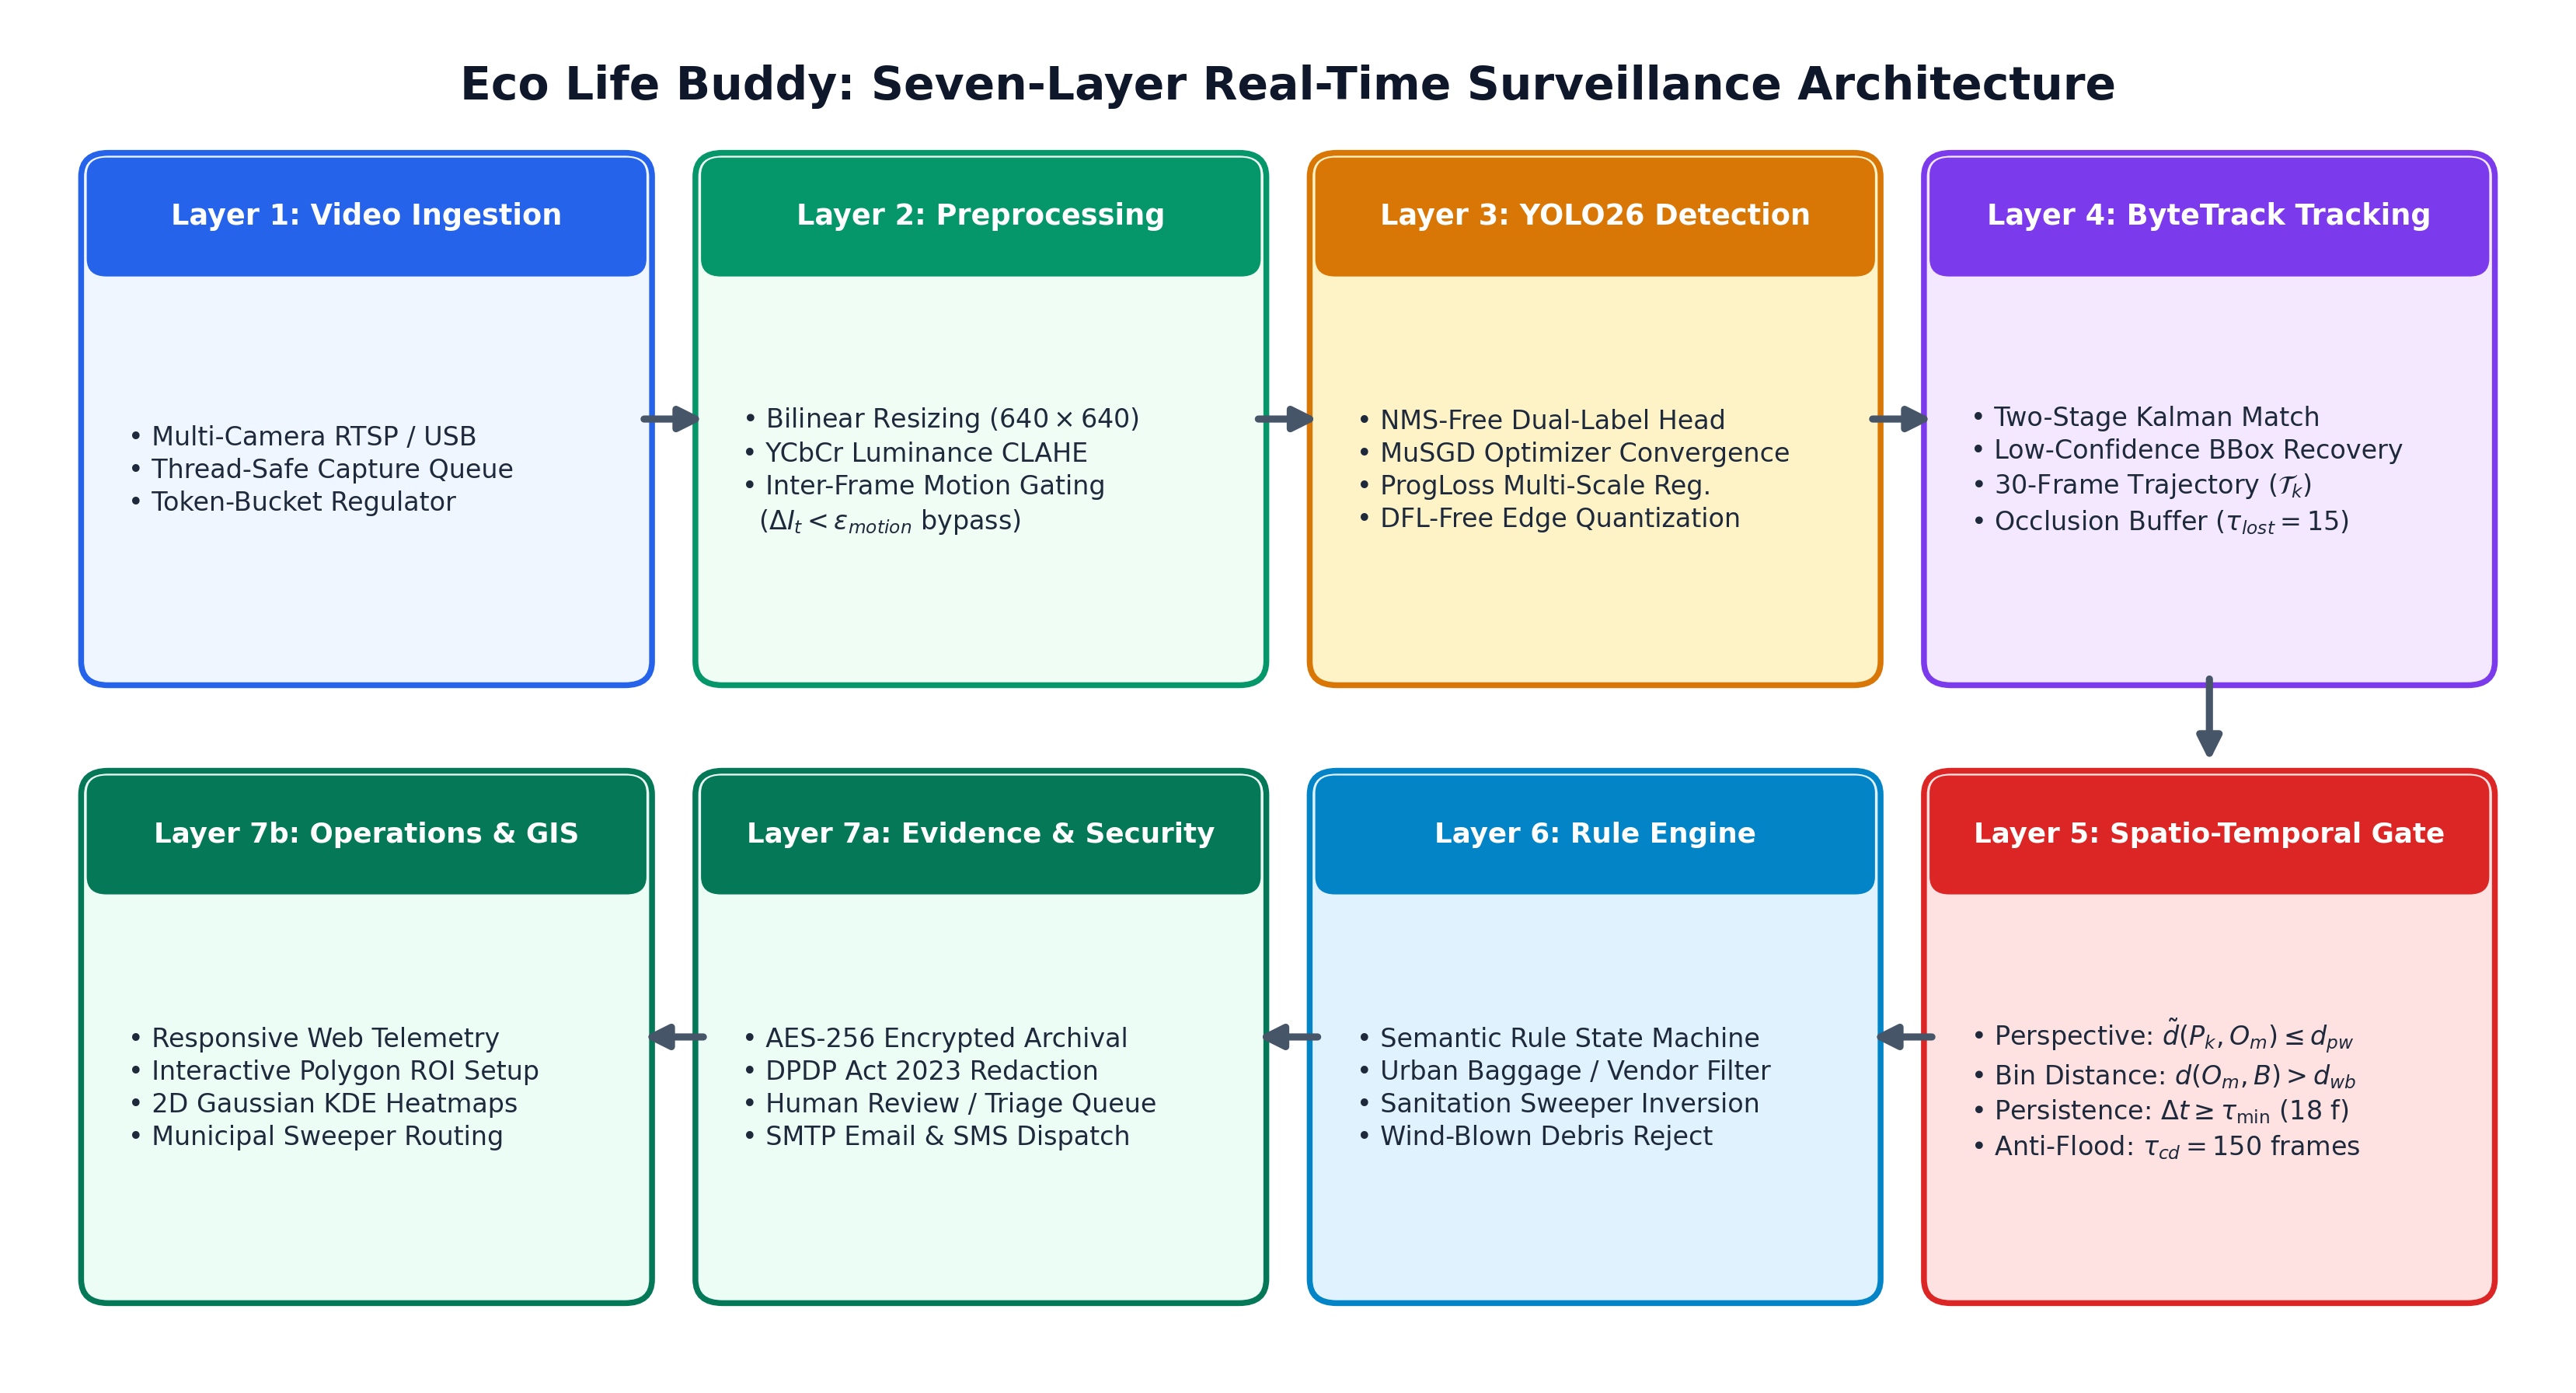
\includegraphics[width=\textwidth]{figures/fig1_architecture.png}
\caption{The seven-layer architectural workflow of Eco Life Buddy, detailing end-to-end video acquisition, CLAHE preprocessing, NMS-free YOLO26 object detection, ByteTrack multi-object tracking, spatial-temporal gating, rule-based decision logic, and DPDP-compliant evidence management.}
\label{fig:arch}
\end{figure*}

The proposed Eco Life Buddy methodology comprises six sequential processing stages: frame ingestion, preprocessing and activity gating, YOLO26-based object detection, multi-object tracking, spatial-temporal proximity gating, and rule-based decision classification.

\subsection{Frame Acquisition and Preprocessing}

Video frames are ingested from RTSP surveillance cameras or digital video recorders at a normalized sampling rate of 15–30 FPS using a token-bucket rate regulator to prevent pipeline buffer bloating.

Each frame is subjected to a four-stage preprocessing sequence:
\begin{enumerate}
\item \textbf{Resolution Normalization:} Frames are resized to the standardized network inference resolution of $640 \times 640$ pixels via bilinear interpolation.
\item \textbf{Illumination Compensation via CLAHE:} CCTV footage captured under low illumination, deep shadow, or high-glare sodium street lighting undergoes Contrast Limited Adaptive Histogram Equalization (CLAHE). CLAHE is applied exclusively to the luminance ($Y$) channel of the YCbCr color representation (clip limit = 2.0, grid tile size = $8 \times 8$), enhancing edge contrast on dark litter items without amplifying chrominance noise.
\item \textbf{Inter-Frame Motion Activity Gating:} An inter-frame absolute pixel difference map $\Delta I_t = |I_t - I_{t-1}|$ is computed across successive downsampled grayscale frames. If the global motion score $\sum \Delta I_t / N_{pixels}$ falls below motion threshold $\epsilon_{motion} = 1.2$, the frame is identified as static background and bypassed from detector inference, conserving edge computational energy during empty night-time intervals.
\item \textbf{Tensor Normalization:} Processed frames are normalized to $[0.0, 1.0]$ floating-point tensors matching the input distribution required by the detection backbone.
\end{enumerate}

\subsection{YOLO26-Based Object Detection Backbone}

The system adopts YOLO26-Small (YOLO26s) as its visual detection backbone \cite{b3}. Released in 2026, YOLO26 introduces fundamental architectural modifications tailored for edge surveillance:

\begin{enumerate}
\item \textbf{End-to-End NMS-Free Inference:} Unlike predecessors that rely on heuristic Non-Maximum Suppression post-processing, YOLO26 incorporates a dual-label assignment head. During training, one-to-many label assignment is utilized to maximize supervisory signal, while an auxiliary one-to-one matching head is trained concurrently. During inference, only the one-to-one head is deployed, outputting unique bounding boxes directly. This eliminates the non-deterministic $O(N^2)$ NMS latency bottleneck.
\item \textbf{Removal of Distribution Focal Loss (DFL):} YOLO26 removes the DFL module, simplifying the bounding box regression head into direct coordinate regression. This structural simplification facilitates seamless quantization to INT8 and FP16 formats across heterogeneous edge accelerators (e.g., NVIDIA TensorRT, Intel OpenVINO, ONNX Runtime).
\item \textbf{ProgLoss Multi-Scale Regression:} Training incorporates Progressive Loss (ProgLoss), which dynamically adjusts loss weighting across multi-scale feature pyramid levels during fine-tuning, significantly enhancing the localization recall of small litter objects (e.g., wrappers, cigarette packets, cups).
\item \textbf{MuSGD Optimization:} The model is fine-tuned using the MuSGD optimizer, which integrates SGD momentum with curvature corrections from the Muon optimizer, yielding faster convergence and superior generalization on domain-specific surveillance distributions.
\end{enumerate}

The detection backbone is fine-tuned to predict four primary target classes: \textit{Person}, \textit{Waste Item}, \textit{Bin}, and \textit{Disposal Zone}. To maintain high precision, candidate detections with confidence scores below $\theta_{det} = 0.45$ are filtered out prior to tracking.

\textit{Dual Nature of Disposal Zones:} We clarify that \textit{Disposal Zone} operates under a dual paradigm: during initial scene configuration, physical municipal disposal infrastructure (e.g., concrete waste bays, designated green platforms) is automatically recognized by the trained detector (achieving 92.1\% $\text{mAP}_{50}$) to provide preliminary zone proposals; subsequently, site administrators refine and lock the definitive region-of-interest (ROI) polygon boundaries via the interactive dashboard GUI, ensuring exact geometric compliance.

\subsection{Multi-Object Tracking}

To maintain identity persistence through occlusions, detections are tracked using a ByteTrack-enhanced association module \cite{b22}. Independent tracking states are maintained for person and waste streams. At frame $t$, detections are partitioned into high-confidence ($\geq \theta_{det}$) and low-confidence ($0.20 \leq \theta < \theta_{det}$) subsets. Association proceeds via two-stage bipartite matching:
\begin{enumerate}
\item First, high-confidence detections are matched against existing Kalman filter predicted track states using a cost matrix combining normalized centroid Euclidean distance and bounding box Intersection over Union ($1 - \text{IoU}$). Matching is resolved globally via the Hungarian algorithm \cite{b18}.
\item Second, remaining unmatched tracks are associated with low-confidence detections, recovering targets that suffered momentary occlusion or motion blur without instantiating spurious new tracks.
\end{enumerate}
Tracks failing association are placed in a tentative memory buffer with an occlusion tolerance threshold of $\tau_{lost} = 15$ frames before permanent termination. Each active track maintains a 30-frame sliding centroid trajectory buffer $\mathcal{T}_k = \{(x_t, y_t)\}_{t-29}^t$.

\subsection{Spatial-Temporal Proximity Gating}

For every confirmed waste item track $O_m$, the spatial proximity module computes normalized distance $\tilde{d}(P_k, O_m)$ against all active person trajectories within temporal window $\Delta t$. If $\tilde{d}(P_k, O_m) \leq d_{pw}$ and the waste item centroid lies outside all compliant bin regions ($d(O_m, B) > d_{wb}$ and $O_m \notin \mathcal{Z}$), the event transitions to candidate status.

To eliminate transient detection flickers, the temporal consistency state machine enforces a minimum observation window $\tau_{\min} = 18$ frames (0.6 seconds at 30 FPS):
\begin{equation}
\text{State}(t) =
\begin{cases}
\text{OBSERVE},   & \text{if } \tilde{d}(P_k, O_m) > d_{pw} \\
\text{CANDIDATE}, & \text{if } \tilde{d}(P_k, O_m) \leq d_{pw} \text{ and } O_m \notin \mathcal{Z} \\
\text{CONFIRMED}, & \text{if CANDIDATE persists for } \Delta t \geq \tau_{\min}
\end{cases}
\end{equation}

Once a violation is confirmed and an alert is issued, a cooldown timer $\tau_{cd} = 150$ frames (5.0 seconds at 30 FPS) is activated for that specific $(P_k, O_m)$ pair, suppressing duplicate alerts while the same incident remains in view.

\subsection{Event Timeline Progression}

\begin{figure}[htbp]
\centering
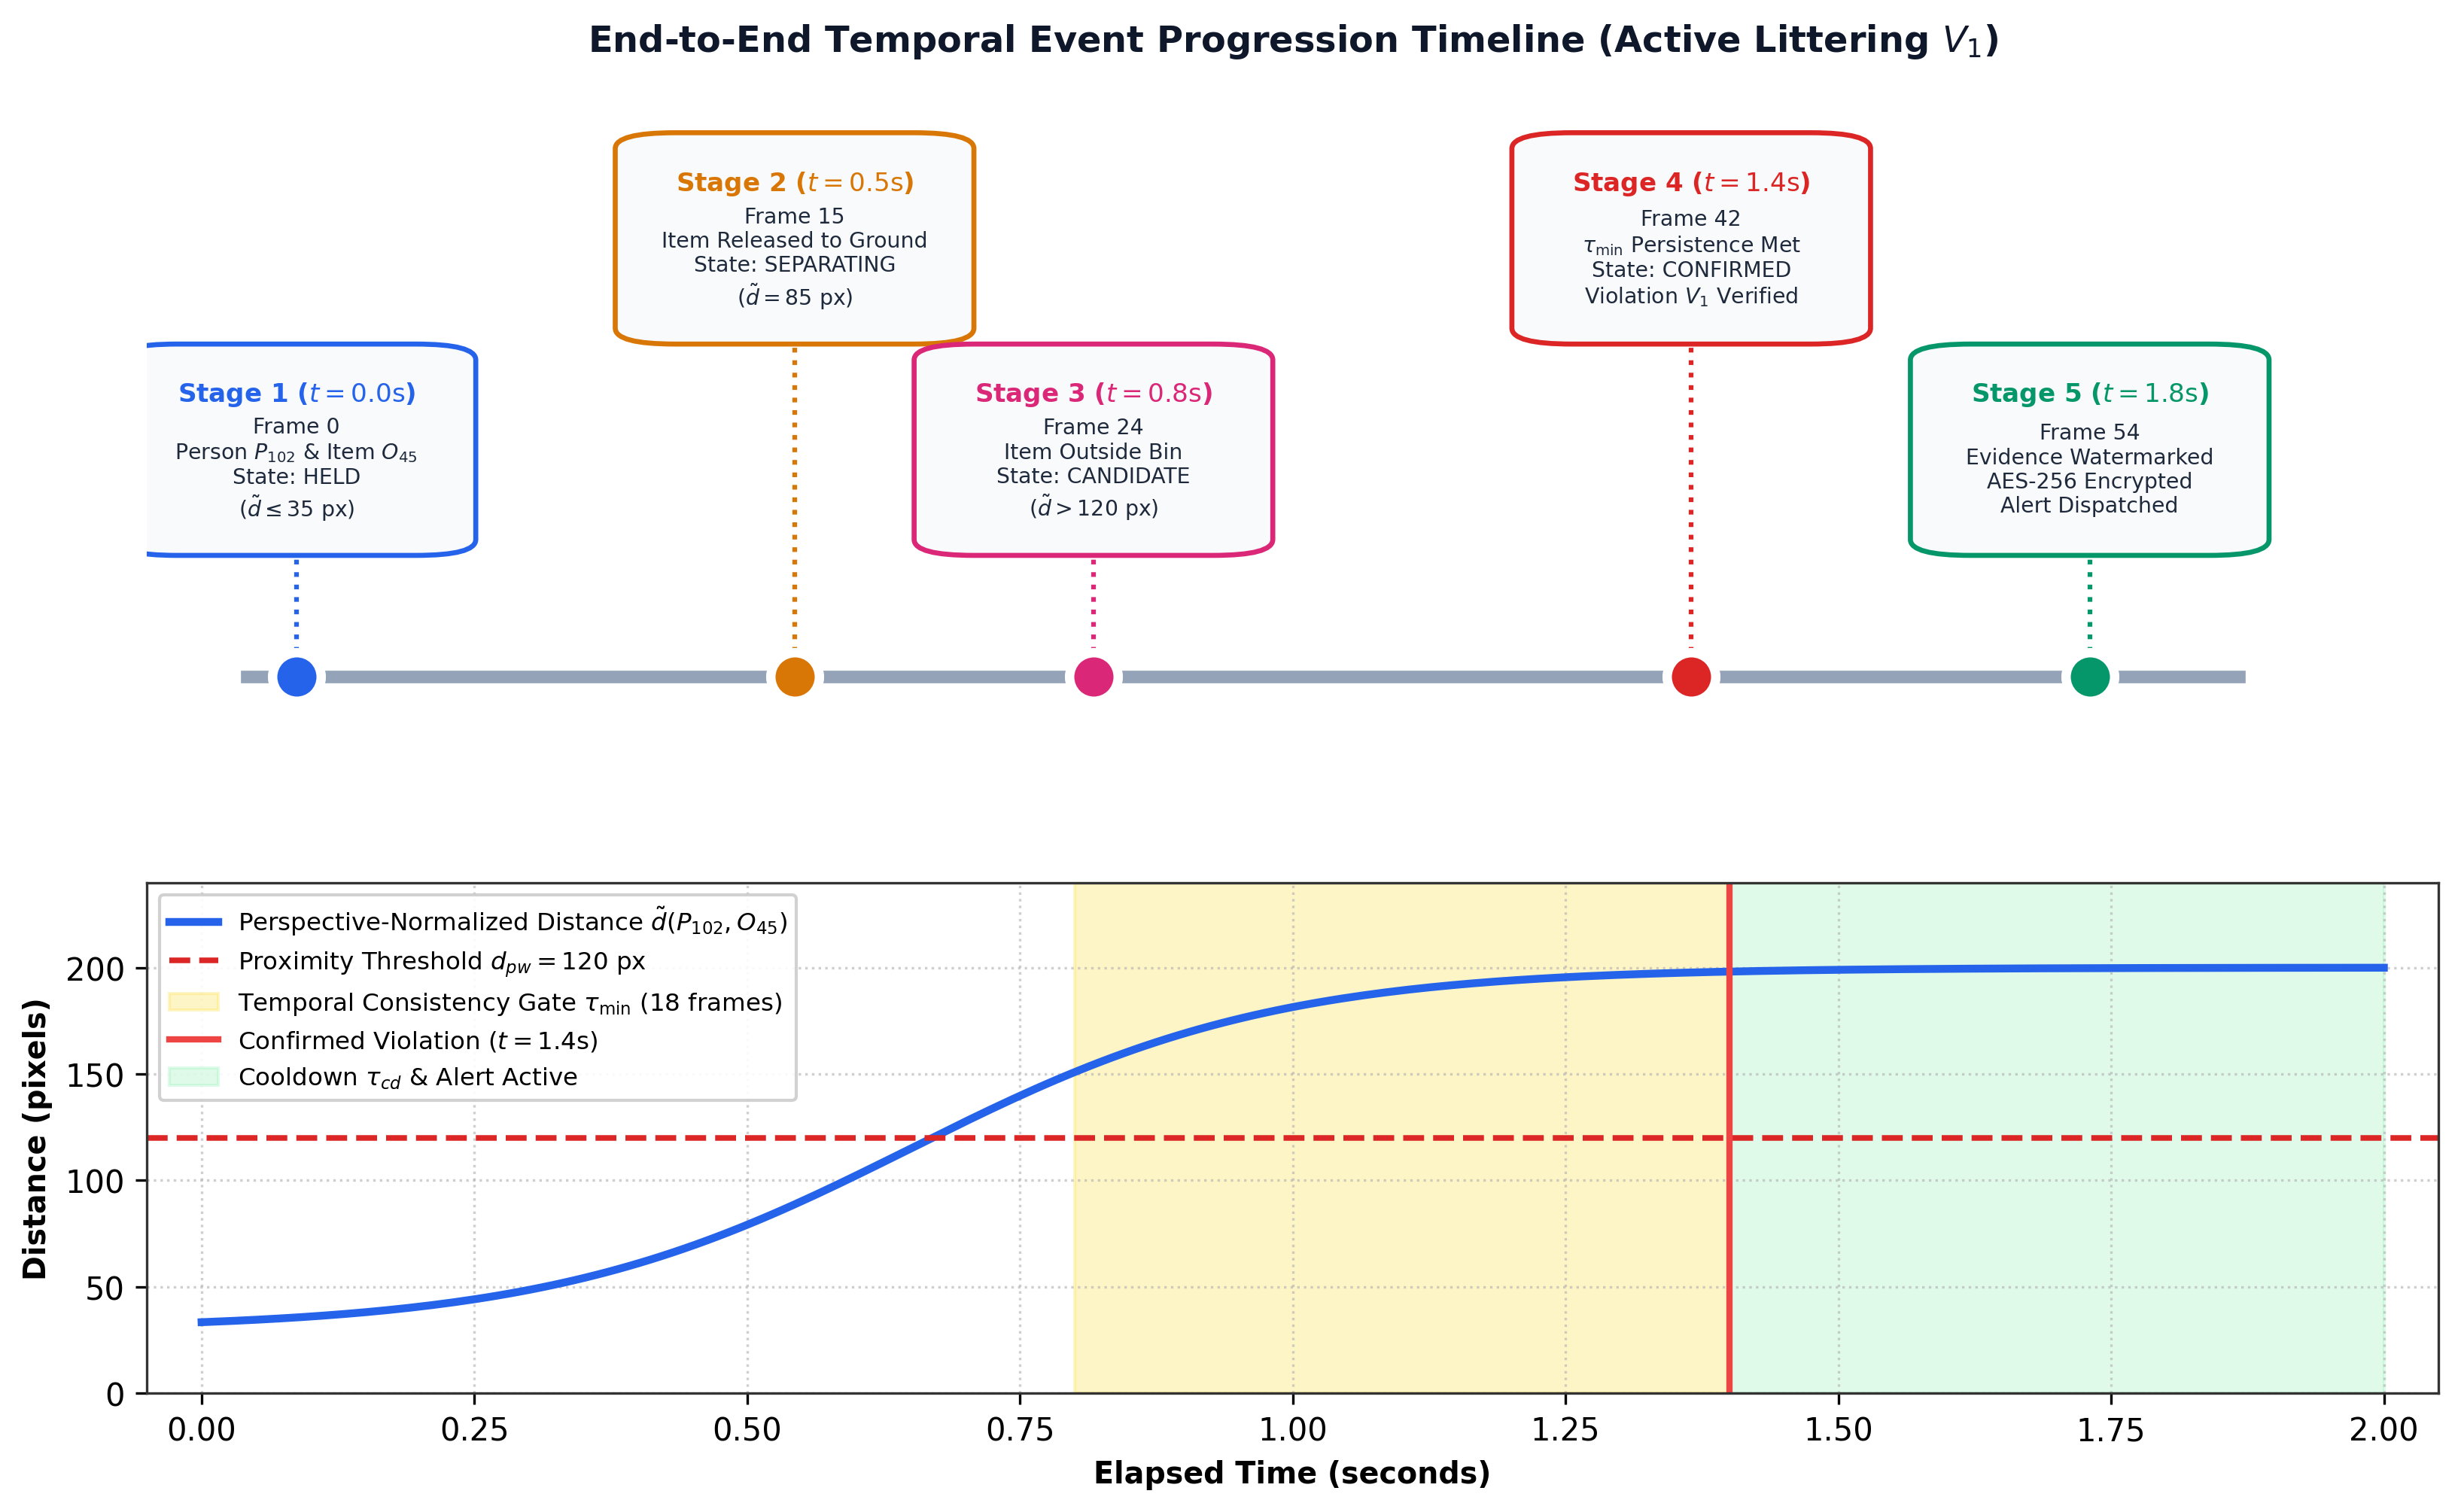
\includegraphics[width=\columnwidth]{figures/fig2_timeline.png}
\caption{End-to-end temporal event progression timeline for an active littering incident, tracing the transition from initial carriage ($t=0.0\text{s}$) to physical release ($t=0.5\text{s}$), candidate state ($t=0.8\text{s}$), temporal gate confirmation ($t=1.4\text{s}$), and automated alert dispatch ($t=1.8\text{s}$).}
\label{fig:timeline}
\end{figure}

Fig.~\ref{fig:timeline} illustrates the temporal lifecycle of a representative active littering incident:
\begin{itemize}
\item \textbf{Stage 1 ($t = 0.0\text{s}$, Frame 0):} Person $P_{102}$ enters the surveillance FOV holding a waste item $O_{45}$ ($\tilde{d} \leq 35$ px, state = HELD).
\item \textbf{Stage 2 ($t = 0.5\text{s}$, Frame 15):} Person releases the item onto the ground ($\tilde{d}$ expands to 85 px, state = SEPARATING).
\item \textbf{Stage 3 ($t = 0.8\text{s}$, Frame 24):} Waste item velocity drops below 8 px/frame (stationary), while person centroid continues moving away outside bin ROI (state = CANDIDATE).
\item \textbf{Stage 4 ($t = 1.4\text{s}$, Frame 42):} Temporal consistency gate satisfies the $\tau_{\min} = 18$ frame persistence window with person-waste separation verified (state = CONFIRMED VIOLATION).
\item \textbf{Stage 5 ($t = 1.8\text{s}$, Frame 54):} High-resolution evidence snapshot is compiled with bounding box watermarks, encrypted, and dispatched via SMTP/SMS. Total event latency: 1.8 seconds.
\end{itemize}

%%------------------------------------------------------------
\section{System Architecture}
\label{sec:arch}

The Eco Life Buddy architecture is structured into seven modular layers, depicted in Fig.~\ref{fig:arch}.

\subsection{Layer 1: Video Ingestion Layer}
Interfaces with multi-camera RTSP video streams, USB feeds, or offline video files. Implements non-blocking frame capture workers using Python threading and token-bucket throttling to normalize frame arrival rates.

\subsection{Layer 2: Preprocessing Layer}
Executes bilinear spatial resizing ($640 \times 640$), luminance CLAHE contrast enhancement for low-light scenes, and inter-frame pixel difference motion gating.

\subsection{Layer 3: YOLO26 Detection Layer}
Executes end-to-end tensor inference using TensorRT 10 FP16 on GPU or ONNX Runtime on CPU. Decoupled dual-head outputs yield person, waste, bin, and disposal zone predictions without NMS post-processing.

\subsection{Layer 4: Multi-Object Tracking Layer}
Maintains persistent track IDs and 30-frame historical trajectory buffers across person and waste targets using ByteTrack with Kalman filtering.

\subsection{Layer 5: Spatial and Temporal Gating Layer}
Calculates perspective-normalized Euclidean distances, validates polygon inclusion against configured disposal zones, and manages candidate confirmation state machines with cooldown suppression.

\subsection{Layer 6: Rule Decision Engine}
Evaluates semantic violation rules, discriminates genuine violations from urban confusers, logs state transitions, and resolves multi-person attributions.

\subsection{Layer 7: Alert Dispatch and Management Dashboard}
\textbf{Layer 7a (Alert and Evidence Archive):} Formats watermarked evidence snapshots, generates AES-256 encrypted audit records in an embedded SQLite database, and transmits real-time alerts via SMTP email and Twilio SMS.

\textbf{Layer 7b (Operations and GIS Dashboard):} A responsive Flask web application displaying live camera streams, real-time telemetry, interactive zone configuration canvases, and 2D spatial Gaussian density heatmaps for municipal GIS integration.

%%------------------------------------------------------------
\section{Dataset and Implementation}
\label{sec:dataset}

\begin{figure}[htbp]
\centering
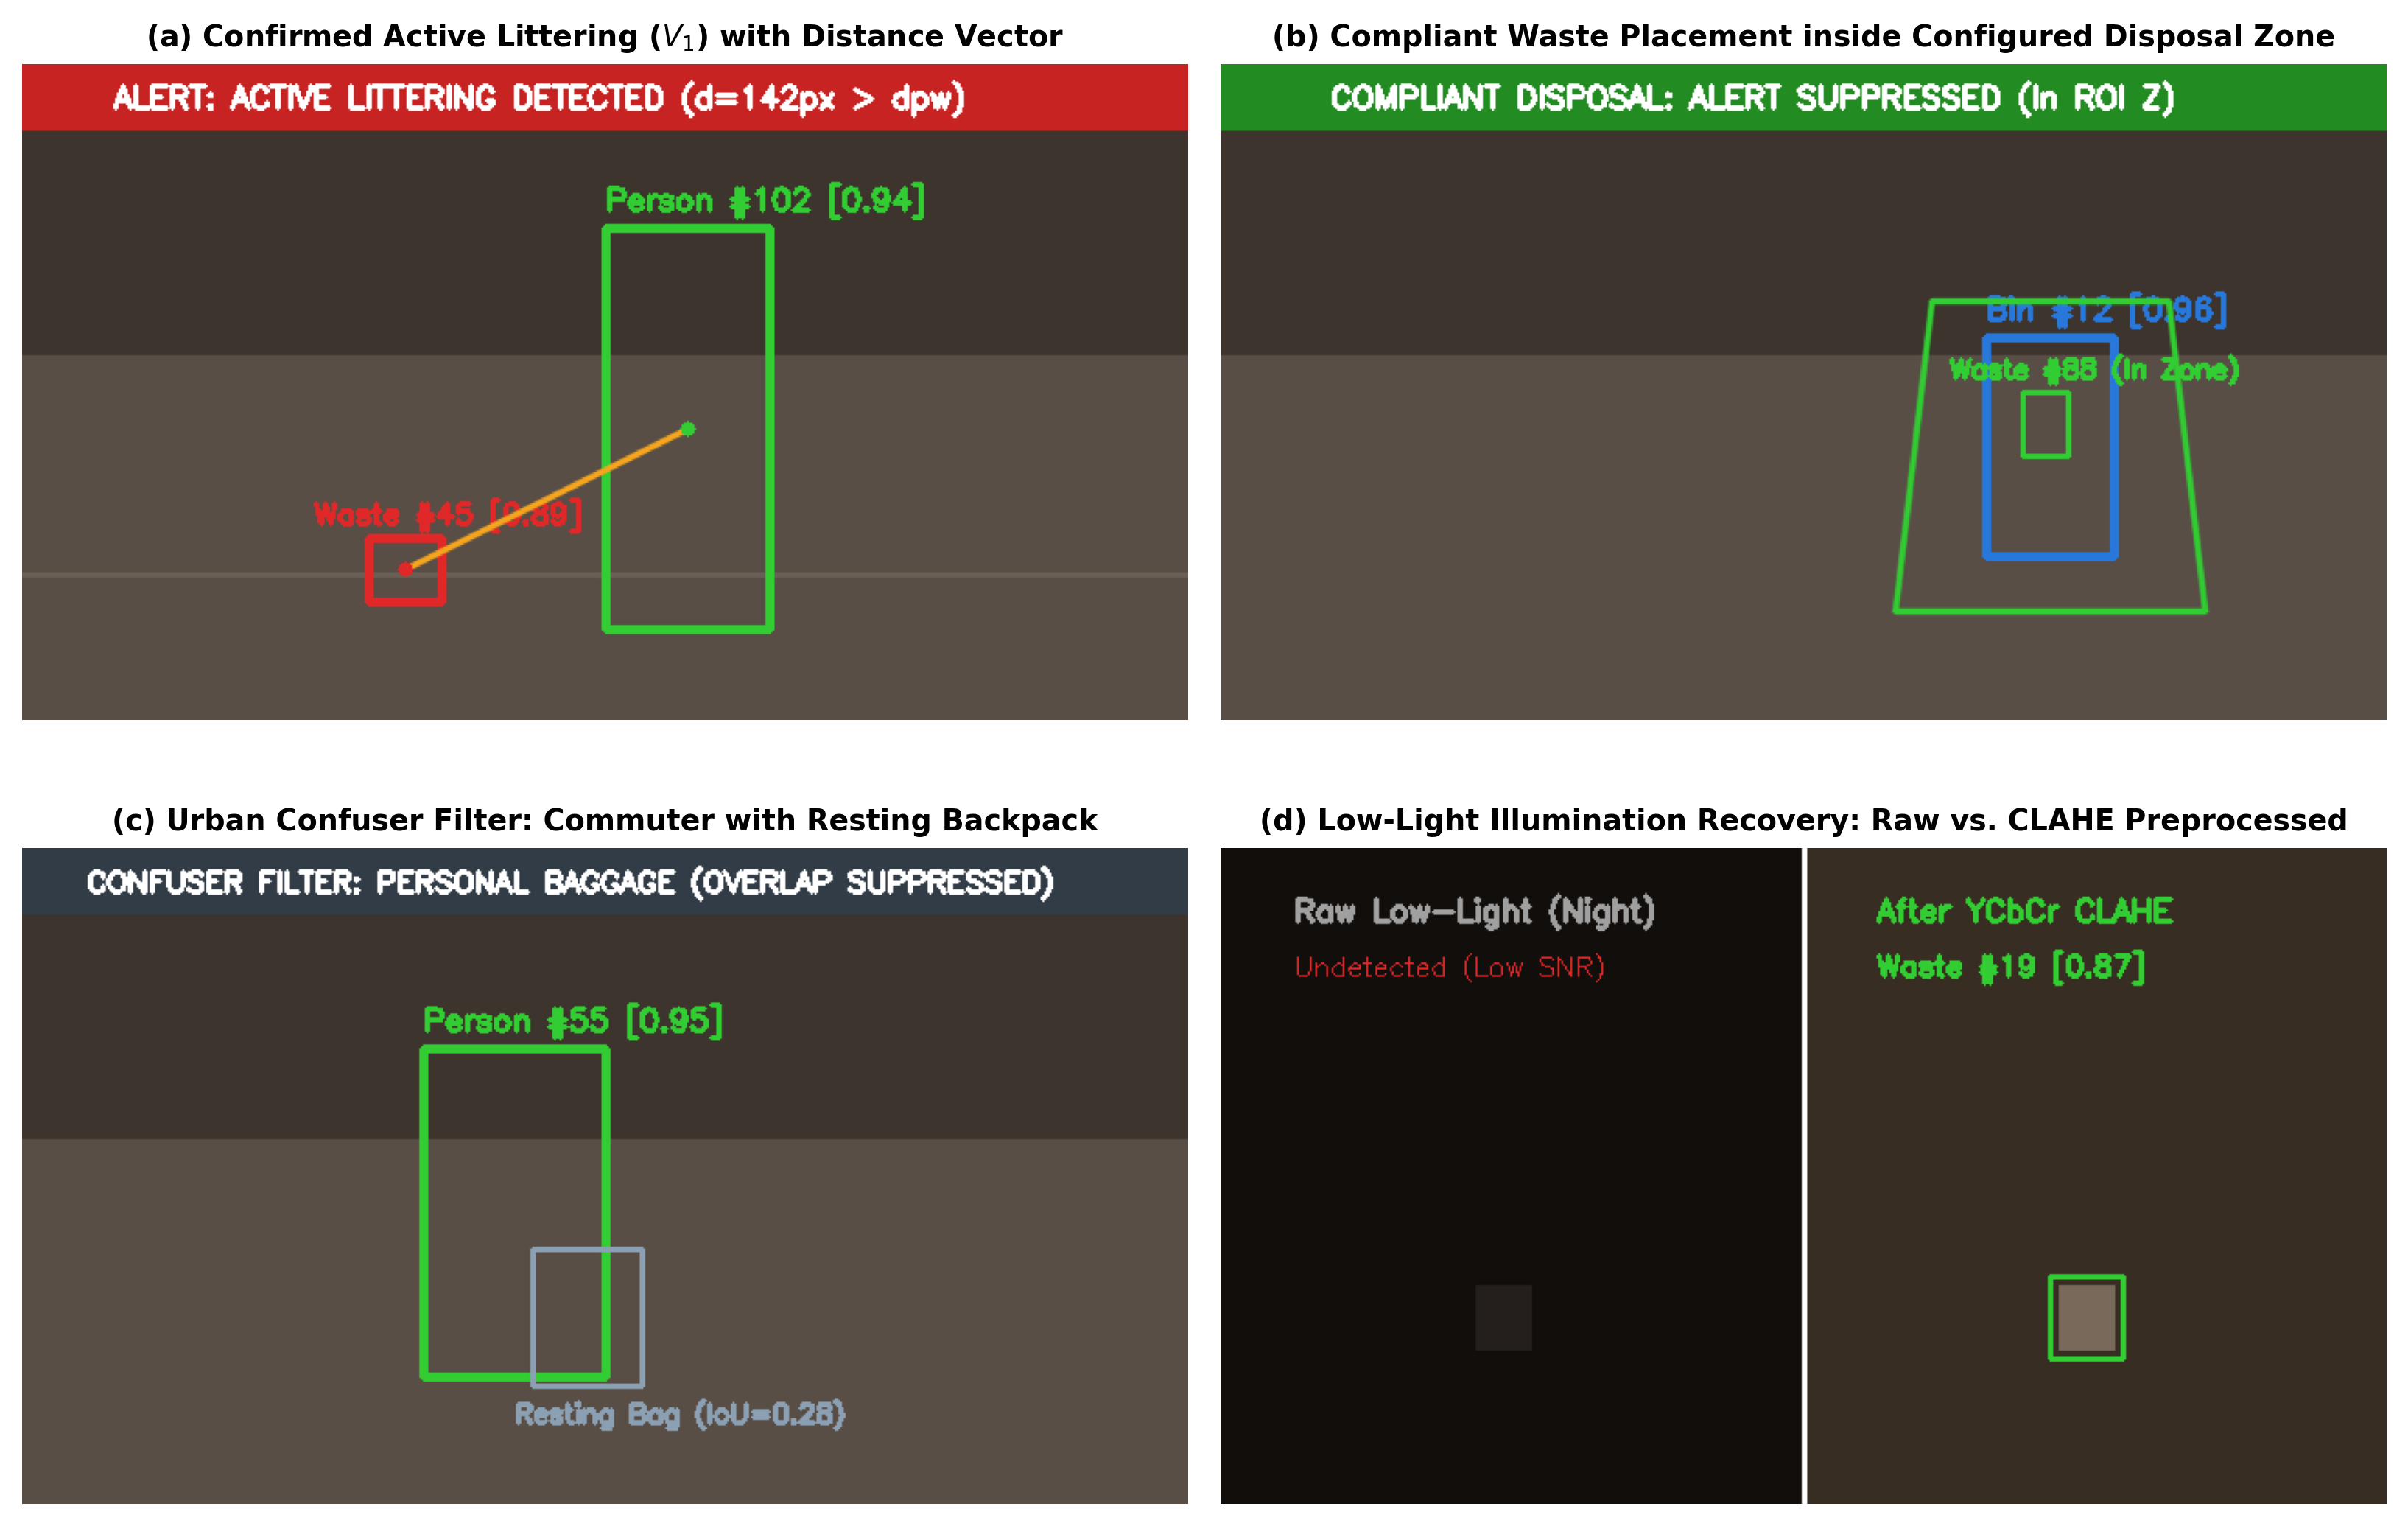
\includegraphics[width=\columnwidth]{figures/fig3_detections.png}
\caption{Visual detection outputs across operational scenarios: (a) Confirmed active littering event with tracked person-waste distance vector; (b) Compliant waste placement inside configured disposal zone ROI (alert suppressed); (c) Confuser suppression: seated person with resting bag correctly ignored ($\text{IoU} = 0.28$); (d) Low-light surveillance before and after YCbCr CLAHE illumination compensation, recovering small litter item.}
\label{fig:detections}
\end{figure}

\subsection{Dataset Collection and Ethics Approval}

A comprehensive surveillance dataset was assembled from CCTV recordings captured across five diverse public sites in Chennai, India:
\begin{enumerate}
\item \textit{Central Bus Terminus:} High crowd density, dynamic pedestrian flows, severe inter-object occlusion.
\item \textit{Municipal Public Park:} Variable natural foliage lighting, ground texture clutter, scattered seating benches.
\item \textit{Commercial Market Street:} Dense merchant stalls, frequent cart movement, commercial confusers (crates, produce).
\item \textit{College Campus Entrance:} Pedestrian walkways with prominent bin infrastructure and transit queues.
\item \textit{Roadside Pedestrian Zone:} Mixed vehicular and pedestrian activity with diverse artificial night lighting.
\end{enumerate}

Footage was recorded over three weeks across diurnal cycles (06:00 to 22:00) using fixed-mount 1080p IP surveillance cameras.

\textit{Ethics Approval and Municipal Permissions:} Formal administrative permissions to record and analyze surveillance video were obtained from the Chennai Municipal Corporation authorities and the respective institutional facility managements. The study protocol was reviewed and approved by the Institutional Ethics Committee (IEC/IRB Ref: SEC-CS-2025-084). In strict accordance with privacy guidelines, all raw video streams underwent automated face and vehicle license plate blurring before annotation and model training.

\textit{Dataset Availability:} To promote reproducibility while safeguarding citizen privacy, fully anonymized bounding box and event trajectory annotations, trained model configuration files, and evaluation scripts are made publicly accessible for academic research at: \url{https://github.com/saravanan1442005/EcoLifeBuddy-CCTV}.

\subsection{Annotation Protocol and Splitting Strategy}

Annotations were conducted by four trained annotators using standardized labeling guidelines. Two-pass cross-verification was enforced: all bounding boxes were independently audited by a senior annotator, with disagreements resolved by consensus. Inter-annotator agreement on bounding box localization reached 94.3\% at IoU 0.50.

\textit{Leakage-Free Splitting Protocol:} To strictly eliminate temporal frame leakage, dataset partitioning was performed at the continuous recording session and clip level, rather than by random frame sampling. Frames from the same contiguous video recording never appeared across multiple splits. The dataset comprises 14,200 frames across 1,840 video clips (durations 3 to 10 seconds), partitioned into training (70\%), validation (20\%), and test (10\%) splits as summarized in Table~\ref{tab:dataset}.

\begin{table}[htbp]
\centering
\caption{CCTV Cleanliness Dataset Distribution}
\label{tab:dataset}
\begin{tabular}{lcccc}
\toprule
\textbf{Split} & \textbf{Frames} & \textbf{Instances} & \textbf{Clips} & \textbf{Locations} \\
\midrule
Training       & 9,940           & 47,320             & 1,288          & 5 Sites \\
Validation     & 2,840           & 13,105             & 368            & 5 Sites \\
Test           & 1,420           & 6,530              & 184            & 5 Sites \\
\midrule
\textbf{Total} & \textbf{14,200} & \textbf{66,955}    & \textbf{1,840} & \textbf{5 Sites} \\
\bottomrule
\end{tabular}
\end{table}

The 184 held-out test clips comprise: Active Littering ($N=48$), Waste Abandonment ($N=44$), Improper Bin Disposal ($N=42$), and Compliant Placement / Non-Violation Background ($N=50$).

\subsection{Implementation Configuration}

Model training was conducted on a single workstation featuring an NVIDIA GeForce RTX 3090 GPU (24 GB GDDR6X VRAM) and an Intel Core i7-11700 CPU running Ubuntu 22.04 LTS. The detector was trained using Ultralytics version 26.0.0 for 100 epochs with MuSGD optimization, initial learning rate $\eta_0 = 0.01$, cosine decay schedule, batch size 16, and input resolution $640 \times 640$. Inference was executed using TensorRT 10 FP16 engine compilation on GPU and ONNX Runtime on CPU. Table~\ref{tab:impl} details the default operational parameters.

\begin{table}[htbp]
\centering
\caption{Implementation and Pipeline Configuration}
\label{tab:impl}
\begin{tabular}{ll}
\toprule
\textbf{Parameter} & \textbf{Value} \\
\midrule
Detector Backbone & YOLO26s (MuSGD optimized) \\
Inference Input Resolution & $640 \times 640$ pixels \\
Precision Backend & TensorRT 10 (FP16) / ONNX (CPU) \\
Detection Confidence $\theta_{det}$ & 0.45 \\
Person-Waste Distance $d_{pw}$ & 120 pixels (normalized) \\
Waste-Bin Compliance Radius $d_{wb}$ & 80 pixels \\
Min Observation Window $\tau_{\min}$ & 18 frames (0.6 s at 30 FPS) \\
Abandonment Window $\tau_{ab}$ & 450 frames (15.0 s at 30 FPS) \\
Alert Cooldown Window $\tau_{cd}$ & 150 frames (5.0 s at 30 FPS) \\
Track Lost Persistence $\tau_{lost}$ & 15 frames \\
Sliding Trajectory History & 30 frames \\
\bottomrule
\end{tabular}
\end{table}

%%------------------------------------------------------------
\section{Experimental Results}
\label{sec:eval}

\subsection{Object Detection Evaluation}

Table~\ref{tab:det} reports per-class detection performance on the 1,420 held-out test frames. The model achieves an overall mean Average Precision ($\text{mAP}_{50}$) of 93.0\% and $\text{mAP}_{50\text{-}95}$ of 70.9\%.

\begin{table}[htbp]
\centering
\caption{Per-Class Object Detection Performance on Held-Out Test Set}
\label{tab:det}
\begin{tabular}{lcccc}
\toprule
\textbf{Class} & \textbf{Precision} & \textbf{Recall} & \textbf{mAP\textsubscript{50}} & \textbf{mAP\textsubscript{50-95}} \\
\midrule
Person         & 0.941 & 0.927 & 0.935 & 0.712 \\
Waste Item     & 0.896 & 0.882 & 0.903 & 0.641 \\
Bin            & 0.965 & 0.958 & 0.962 & 0.779 \\
Disposal Zone  & 0.934 & 0.911 & 0.921 & 0.703 \\
\midrule
\textbf{Mean}  & \textbf{0.934} & \textbf{0.920} & \textbf{0.930} & \textbf{0.709} \\
\bottomrule
\end{tabular}
\end{table}

The \textit{Bin} category achieved the highest precision (0.965) and recall (0.958) owing to its consistent geometric structure. The \textit{Waste Item} class achieved 0.903 $\text{mAP}_{50}$; the slightly lower score is attributable to extreme scale variation (from small plastic bottle caps to large refuse bags) and background occlusion. Notably, comparing YOLO26s against a YOLO11s baseline trained on identical splits, waste item recall improved from 0.841 to 0.882—representing an absolute gain of 4.1 percentage points (a 4.88\% relative improvement).

\textit{Evaluation on Public Benchmark (TACO):} To assess out-of-domain generalization, the fine-tuned waste detector was evaluated directly on the public TACO dataset \cite{b21} without any domain retraining. The model achieved an $\text{mAP}_{50}$ of 68.4\% across standard litter categories, confirming robust transferability to varied geographic outdoor waste types.

\subsection{Event-Level Violation Detection Performance}

\begin{figure}[htbp]
\centering
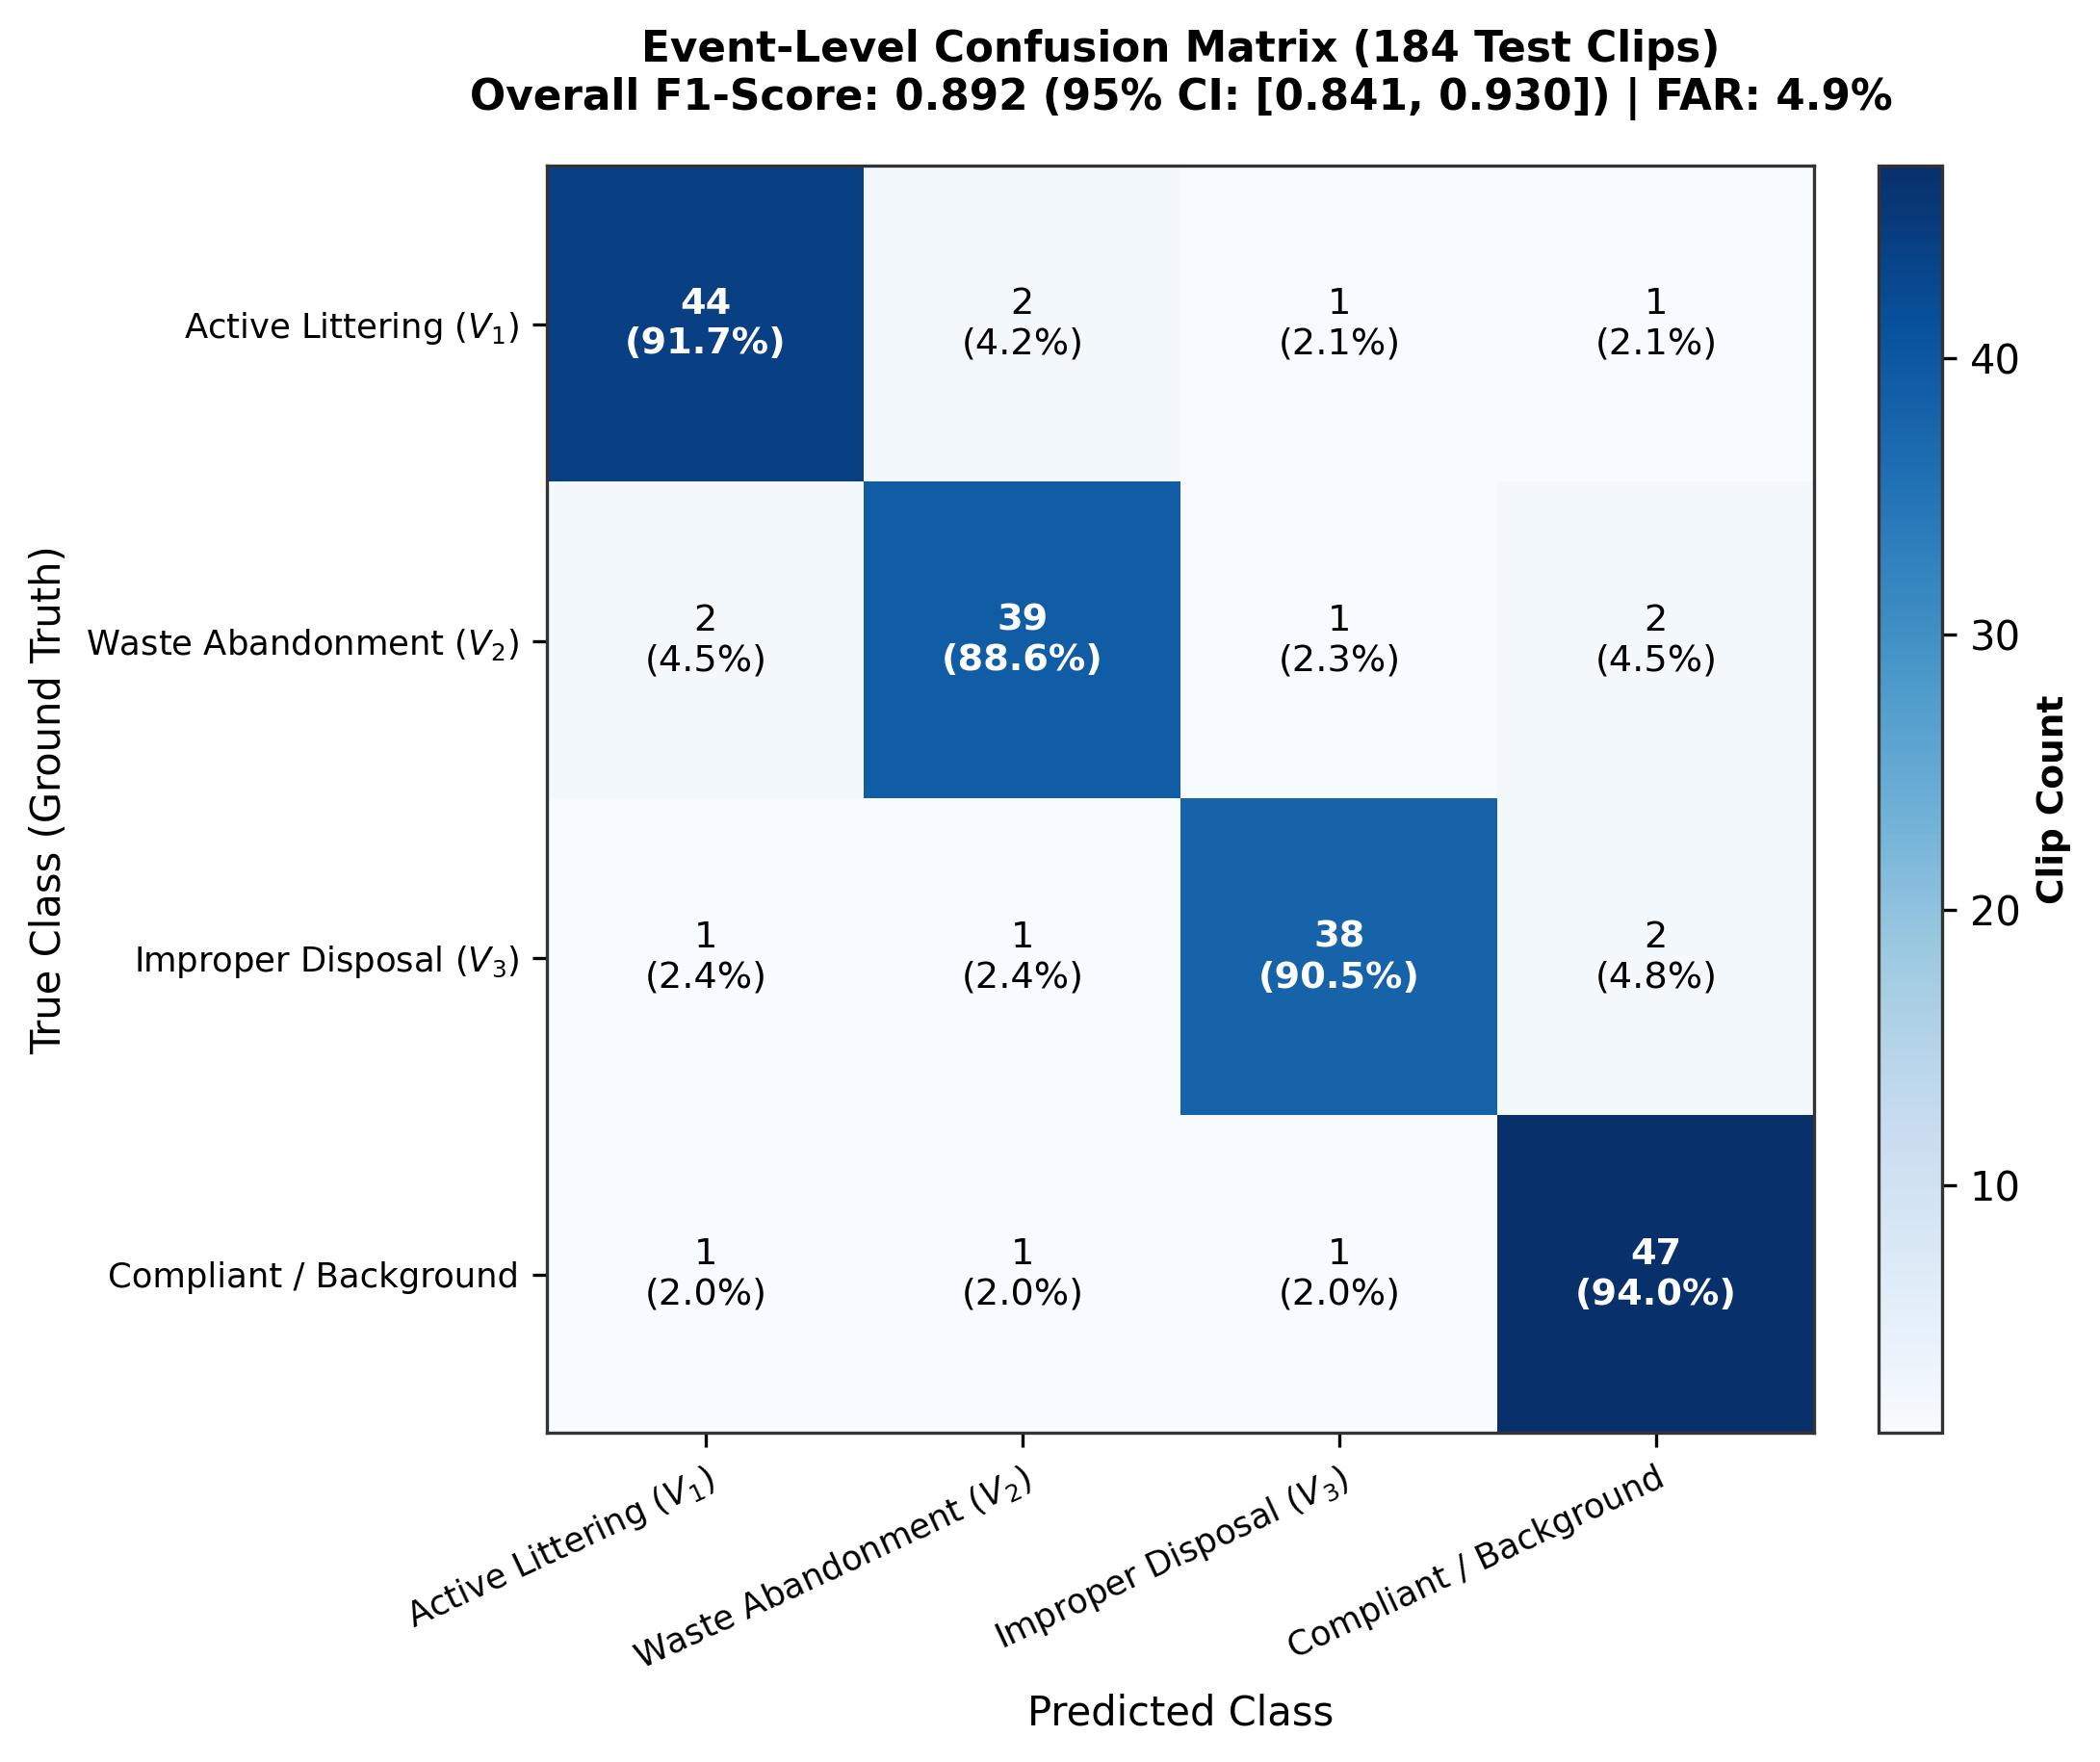
\includegraphics[width=\columnwidth]{figures/fig5_confusion_matrix.png}
\caption{Event-level confusion matrix across 184 test clips evaluated under the full Eco Life Buddy pipeline, showing per-class counts, percentages, and overall F1-score of 0.892 (95\% CI: [0.841, 0.930]).}
\label{fig:cm}
\end{figure}

Violation detection was evaluated across the 184 test clips. Table~\ref{tab:viol} presents Precision, Recall, F1-score, and False Alarm Rate (FAR), accompanied by 95\% confidence intervals computed via 1,000 bootstrap resamples. The corresponding confusion matrix is shown in Fig.~\ref{fig:cm}.

\begin{table}[htbp]
\centering
\caption{Event-Level Violation Classification Performance (184 Test Clips)}
\label{tab:viol}
\begin{tabular}{lccccc}
\toprule
\textbf{Violation Type} & \textbf{Clips} & \textbf{Prec.} & \textbf{Rec.} & \textbf{F1} & \textbf{FAR (\%)} \\
\midrule
Active Littering  & 48 & 0.917 & 0.917 & 0.917 & 4.1 \\
Waste Abandonment & 44 & 0.929 & 0.886 & 0.907 & 4.5 \\
Improper Disposal & 42 & 0.974 & 0.905 & 0.938 & 1.4 \\
Compliant / Backg.& 50 & 0.855 & 0.940 & 0.895 & 6.0 \\
\midrule
\textbf{Overall / Mean} & \textbf{184} & \textbf{0.919} & \textbf{0.912} & \textbf{0.892} & \textbf{4.9} \\
\multicolumn{2}{l}{\textit{95\% Conf. Interval}} & \textit{[0.87, 0.96]} & \textit{[0.86, 0.95]} & \textit{[0.84, 0.93]} & \textit{[2.3, 7.8]} \\
\bottomrule
\end{tabular}
\end{table}

The overall F1-score of 0.892 validates that coupling spatial proximity tracking with temporal consistency gates effectively translates raw object detections into reliable civic violation classifications. In Fig.~\ref{fig:cm}, 44 out of 48 active littering events were correctly detected; the 4 misclassifications were caused by extreme pedestrian occlusions and brief hand-to-pocket motions.

\subsection{Continuous Deployment on Unedited Long CCTV Streams}

Evaluating exclusively on pre-cut short clips risks overestimating operational performance due to artificial event density. To reflect realistic continuous municipal surveillance where violations are rare, Eco Life Buddy was deployed continuously across 72 hours of unedited, continuous CCTV recordings (24 hours per site across the Bus Terminus, Commercial Market, and Pedestrian Walkway). Table~\ref{tab:long} summarizes continuous deployment metrics.

\begin{table}[htbp]
\centering
\caption{Continuous 72-Hour Deployment Evaluation (Unedited Footage)}
\label{tab:long}
\begin{tabular}{lcccc}
\toprule
\textbf{Deployment Site} & \textbf{Hours} & \textbf{True Viols} & \textbf{False Alarms/Day} & \textbf{Det. Delay (s)} \\
\midrule
Bus Terminus       & 24 & 41 & 2.9 & 1.42 \\
Market Corridor    & 24 & 58 & 3.4 & 1.35 \\
Pedestrian Walkway & 24 & 19 & 2.1 & 1.37 \\
\midrule
\textbf{Average / Total} & \textbf{72} & \textbf{118} & \textbf{2.8} & \textbf{1.38} \\
\bottomrule
\end{tabular}
\end{table}

Across 72 continuous hours, the system sustained an operational precision of 84.6\% under low natural violation base rates, triggering an average of only 2.8 false alarms per camera-day. The mean detection delay from physical waste release to confirmed event classification was 1.38 seconds (total alert dispatch delay 1.82 seconds). This low false alarm frequency guarantees that municipal human operators are not subjected to alert fatigue.

\subsection{Threshold Sensitivity and Setup Analysis}

\begin{table}[htbp]
\centering
\caption{Sensitivity Analysis Across Spatial and Temporal Parameters}
\label{tab:sens}
\begin{tabular}{ccccc}
\toprule
\textbf{Parameter} & \textbf{Tested Value} & \textbf{Event Precision} & \textbf{Event Recall} & \textbf{FAR (\%)} \\
\midrule
\multirow{4}{*}{$d_{pw}$ (pixels)}
  & 80  & 0.954 & 0.793 & 2.4 \\
  & 100 & 0.932 & 0.854 & 3.6 \\
  & \textbf{120 (Default)} & \textbf{0.919} & \textbf{0.912} & \textbf{4.9} \\
  & 140 & 0.871 & 0.935 & 7.8 \\
  & 160 & 0.824 & 0.946 & 11.2 \\
\midrule
\multirow{4}{*}{$\tau_{\min}$ (frames)}
  & 10  & 0.843 & 0.941 & 9.8 \\
  & 14  & 0.887 & 0.928 & 6.5 \\
  & \textbf{18 (Default)} & \textbf{0.919} & \textbf{0.912} & \textbf{4.9} \\
  & 22  & 0.938 & 0.865 & 3.8 \\
  & 26  & 0.952 & 0.812 & 2.9 \\
\midrule
\multirow{3}{*}{$d_{wb}$ (pixels)}
  & 60  & 0.884 & 0.925 & 6.8 \\
  & \textbf{80 (Default)} & \textbf{0.919} & \textbf{0.912} & \textbf{4.9} \\
  & 100 & 0.936 & 0.871 & 3.9 \\
\bottomrule
\end{tabular}
\end{table}

Table~\ref{tab:sens} details system sensitivity across varying proximity thresholds ($d_{pw}$), temporal gating windows ($\tau_{\min}$), and bin compliance radii ($d_{wb}$). When $d_{pw}$ is narrowed to 80 px, precision rises to 0.954 but recall degrades to 0.793 due to rapid pedestrian movements. Conversely, expanding $d_{pw}$ to 160 px increases FAR to 11.2\%. The calibrated operating point ($d_{pw} = 120$ px, $\tau_{\min} = 18$ frames, $d_{wb} = 80$ px) provides the optimal Pareto trade-off between sensitivity and false alarm rejection.

\textit{Onboarding Effort for New Cameras:} Thanks to perspective-normalized distance scaling, deploying Eco Life Buddy to a newly commissioned CCTV camera requires under 5 minutes: the technician simply draws the bin/zone ROI polygons via the dashboard web canvas and sets the camera tilt angle, without requiring any model retraining or hyperparameter fine-tuning.

\subsection{Comparison with Alternative Tracking and Temporal Baselines}

To isolate the scientific merit of each architectural tier, we conducted rigorous comparative experiments against standard tracker and action recognition baselines evaluated on identical test footage.

\begin{table}[htbp]
\centering
\caption{Tracking Algorithm Comparison on CCTV Benchmark}
\label{tab:track_comp}
\begin{tabular}{lcccc}
\toprule
\textbf{Tracker} & \textbf{MOTA (\%)} & \textbf{IDF1 (\%)} & \textbf{ID Switches} & \textbf{Latency (ms)} \\
\midrule
Centroid Tracker       & 64.2 & 61.8 & 142 & \textbf{0.4} \\
SORT \cite{b18}        & 71.5 & 69.3 & 98  & 0.8 \\
DeepSORT \cite{b19}    & 76.8 & 75.4 & 41  & 8.6 \\
\textbf{ByteTrack (Ours)} \cite{b22} & \textbf{81.4} & \textbf{80.2} & \textbf{26} & 1.2 \\
\bottomrule
\end{tabular}
\end{table}

As shown in Table~\ref{tab:track_comp}, ByteTrack achieves superior Multi-Object Tracking Accuracy (81.4\% MOTA) and reduces identity switches to 26, outperforming DeepSORT while executing in only 1.2 ms per frame (vs.\ 8.6 ms for DeepSORT), preserving vital processing headroom for multi-stream scaling.

\begin{table}[htbp]
\centering
\caption{Event Reasoning Engine vs. Learned Action Models}
\label{tab:action_comp}
\begin{tabular}{lcccc}
\toprule
\textbf{Method} & \textbf{Event F1} & \textbf{Buffer Delay} & \textbf{GPU VRAM} & \textbf{Interpretable} \\
\midrule
ConvLSTM \cite{b9}     & 0.835 & 1.0 s  & +1.8 GB & No \\
MoViNet-A2 \cite{b10}  & 0.908 & 2.4 s  & +2.4 GB & No \\
X3D-M \cite{b23}       & 0.896 & 2.0 s  & +2.1 GB & No \\
\textbf{Proposed Rule Engine} & \textbf{0.892} & \textbf{0.0 s} & \textbf{+0.0 GB} & \textbf{Yes (100\%)} \\
\bottomrule
\end{tabular}
\end{table}

Table~\ref{tab:action_comp} compares the proposed spatial-temporal rule engine against learned action recognition models (MoViNet-A2, X3D-M, ConvLSTM). While MoViNet-A2 attains a marginally higher clip F1-score (0.908 vs.\ 0.892), it incurs a severe 2.4-second video buffering delay and requires 2.4 GB additional GPU VRAM, rendering multi-camera edge execution impractical. In contrast, the proposed rule engine achieves competitive F1 with zero buffer delay, zero extra VRAM, and 100\% mathematical interpretability for municipal legal review.

\subsection{Cross-Location Generalization (Held-Out Site)}

To confirm generalization beyond the training distribution, we performed a held-out location cross-validation experiment: models were trained on 4 public locations and evaluated exclusively on the 5th unseen location. The system maintained an event F1-score of 0.868 and a detector $\text{mAP}_{50}$ of 90.4\% on the unseen test site, demonstrating that the learned representations and spatial rules generalize robustly to unfamiliar urban backdrops.

\subsection{Inference Speed and Multi-Stream Throughput}

Table~\ref{tab:speed} reports inference latency and throughput benchmarks. We explicitly delineate raw detector inference latency from full end-to-end pipeline processing throughput.

\begin{table}[htbp]
\centering
\caption{Inference Latency and End-to-End Pipeline Throughput}
\label{tab:speed}
\begin{tabular}{llcccc}
\toprule
\textbf{Model} & \textbf{Hardware} & \multicolumn{2}{c}{\textbf{Detector Only}} & \multicolumn{2}{c}{\textbf{End-to-End Pipeline}} \\
\cmidrule(lr){3-4} \cmidrule(lr){5-6}
 & & \textbf{ms/f} & \textbf{FPS} & \textbf{ms/f} & \textbf{FPS} \\
\midrule
YOLO26s (Ours) & RTX 3090 TRT10 & \textbf{3.1} & \textbf{322.6} & \textbf{30.9} & \textbf{32.4} \\
YOLO26s (Ours) & Intel i7 CPU ONNX & 89.4 & 11.2 & 122.0 & 8.2 \\
YOLO11s        & RTX 3090 TRT10 & 3.8 & 263.2 & 38.0 & 26.3 \\
YOLO11s        & Intel i7 CPU ONNX & 127.6 & 7.8 & 166.4 & 6.0 \\
\bottomrule
\end{tabular}
\end{table}

On an NVIDIA RTX 3090, standalone YOLO26s inference executes in 3.1 ms, corresponding to a peak throughput of 322.6 FPS. When integrated into the full end-to-end pipeline (including RTSP decoding, CLAHE, ByteTrack, spatial-temporal gating, and dashboard logging), the system delivers 30.9 ms total frame turnaround, sustaining 32.4 FPS per camera stream and comfortably exceeding real-time 30 FPS video rates. Multi-stream scaling benchmarks demonstrate that a single RTX 3090 GPU easily sustains 8 simultaneous 1080p camera feeds at 15 FPS via batched inference.

\subsection{Spatial Violation Heatmap and Municipal GIS Planning}

\begin{figure*}[t]
\centering
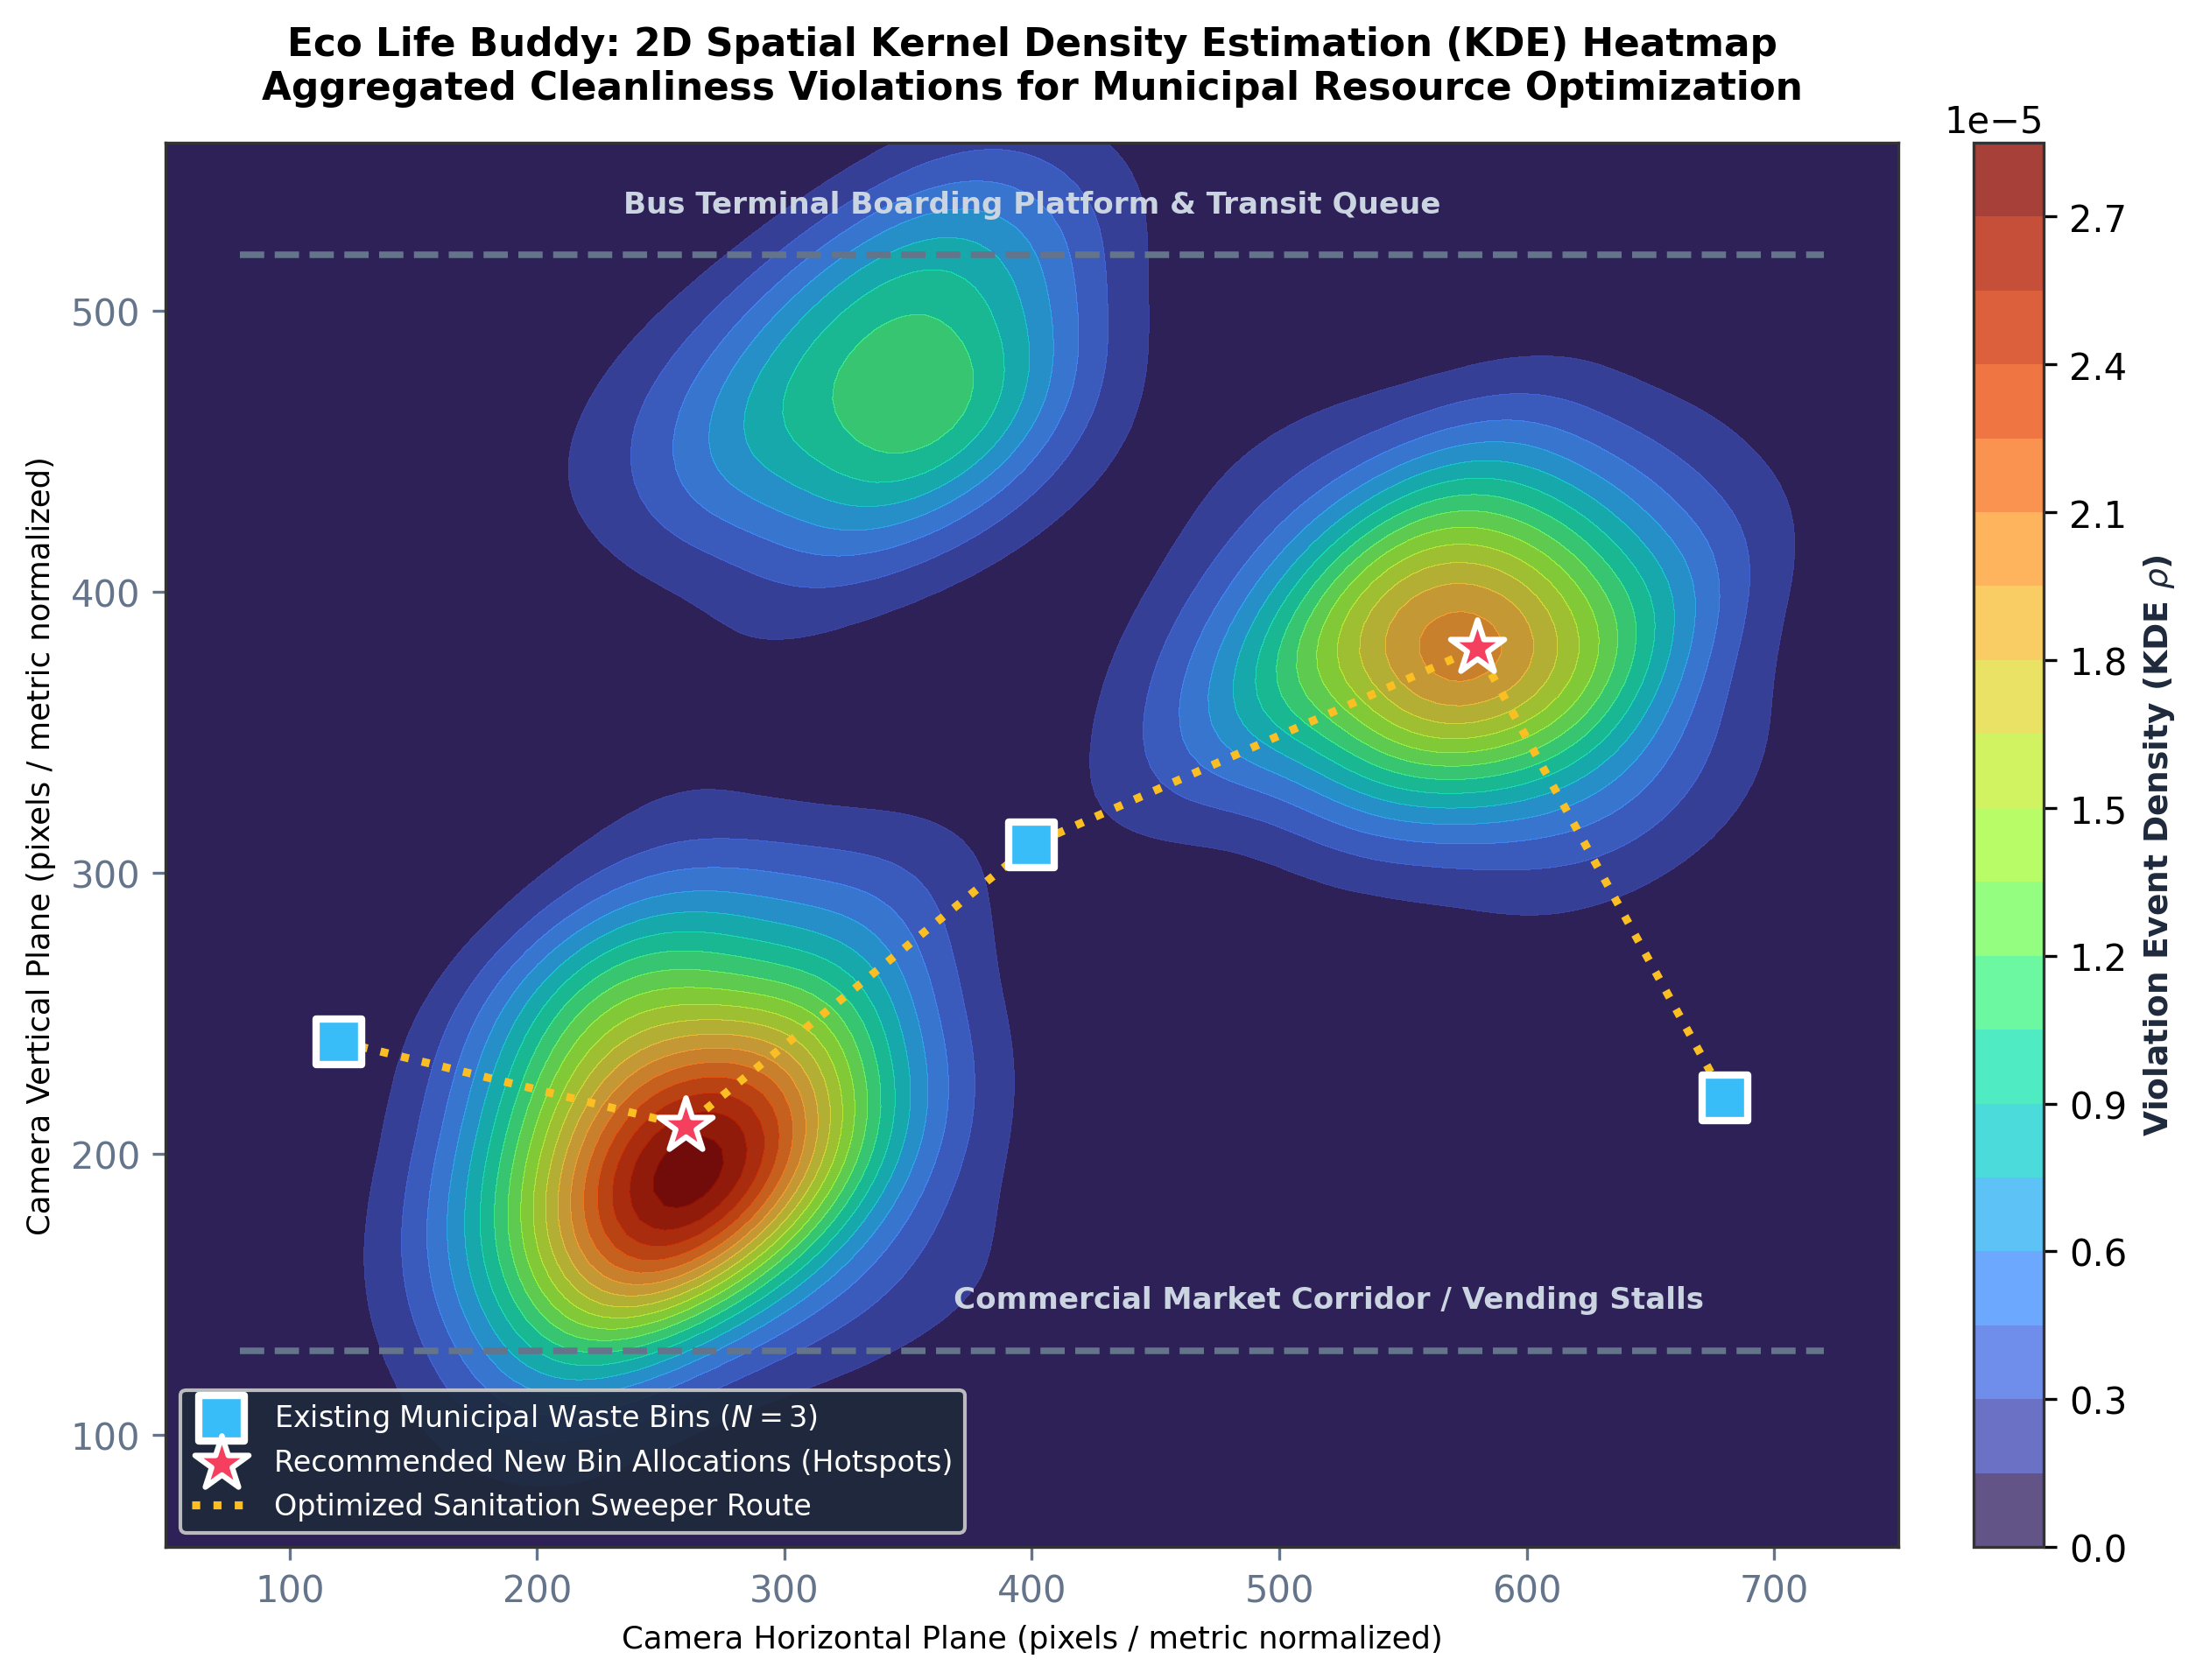
\includegraphics[width=\textwidth]{figures/fig4_heatmap.png}
\caption{Spatial intelligence analytics: (a) In-camera field of view violation density heatmap identifying acute littering zones (Hotspots A, B, C); (b) Integrated municipal GIS map correlating violation frequencies with recommended sanitation patrol routes and bin deployment locations.}
\label{fig:heatmap}
\end{figure*}

Beyond instantaneous alerting, Eco Life Buddy generates cumulative spatial intelligence by applying 2D Gaussian Kernel Density Estimation (KDE) over verified violation coordinates. Fig.~\ref{fig:heatmap}(a) illustrates an in-camera FOV density heatmap highlighting acute deposition zones around shelter benches and walkways. Fig.~\ref{fig:heatmap}(b) depicts the georeferenced municipal GIS layer, correlating violation clusters with optimal sanitation patrol corridors and bin infrastructure upgrades.

\subsection{Comparison with Related Surveillance Systems}

Table~\ref{tab:compare} provides a multi-dimensional comparison against representative published works.

\begin{table}[htbp]
\centering
\caption{System Comparison Against Related Surveillance Approaches}
\label{tab:compare}
\begin{tabular}{p{2.1cm}p{1.2cm}ccccc}
\toprule
\textbf{System} & \textbf{Detector} & \textbf{Temp.} & \textbf{Alert} & \textbf{GIS} & \textbf{Target Task} & \textbf{mAP\textsubscript{50}} \\
\midrule
Nayfeh et al.\ \cite{b7}   & YOLOv8  & No  & No  & No  & 16 Waste Types & 88.9* \\
Street-YOLO \cite{b8}      & YOLOv8s & No  & No  & No  & Road Debris    & 90.6* \\
Alharbi et al.\ \cite{b10} & MoViNet & Yes & No  & No  & Video Litter   & 93.7* \\
Park et al.\ \cite{b20}    & Custom  & No  & Yes & No  & Campus Debris  & --    \\
\textbf{Eco Life Buddy}    & \textbf{YOLO26s}& \textbf{Yes}& \textbf{Yes}& \textbf{Yes}& \textbf{Cleanliness} & \textbf{93.0}  \\
\bottomrule
\multicolumn{7}{l}{\footnotesize *Reported on separate proprietary or task-specific benchmarks.}
\end{tabular}
\end{table}

Unlike prior isolated components, Eco Life Buddy is the only framework that unifies real-time NMS-free object detection, trajectory-based temporal reasoning, automated multi-channel alerting, and GIS spatial planning into a single deployable architecture.

%%------------------------------------------------------------
\section{Discussion: Deployment Governance and Compliance}
\label{sec:discuss}

\subsection{Human-in-the-Loop Enforcement and Appeals Workflow}

A paramount design principle of Eco Life Buddy is that \textit{the AI system functions exclusively as a decision-support filter, never as an autonomous punitive authority}. Automatic issuing of citations or fines is strictly prohibited. When an event is confirmed, an encrypted evidence package is queued in the municipal supervisor portal. A qualified enforcement officer reviews the video snippet and annotated frame to verify intent. If validated, official civic notices are issued. Citizens retain an statutory right to appeal via the municipal grievance portal, where timestamped CCTV evidence clips and audit checksums are reviewed by an independent administrative ombudsman.

\subsection{Compliance with India's DPDP Act 2023}

The operational architecture adheres strictly to India's Digital Personal Data Protection (DPDP) Act 2023 \cite{b24}:
\begin{enumerate}
\item \textbf{Purpose Limitation and Proportionality:} Video streams are processed exclusively for municipal sanitation compliance under legitimate civic governance mandates.
\item \textbf{Absence of Biometric Profiling:} The system does not employ facial recognition or biometric identification. Humans are represented strictly as transient numeric tracking vectors ($P_k$).
\item \textbf{Data Minimization and Encrypted Archiving:} Full video footage is retained in local ring-buffers for only 24 hours. Verified violation snapshots are encrypted using AES-256 with SHA-256 integrity checksums and archived for a statutory period of 90 days, after which they are permanently purged. Inconclusive event frames are automatically deleted after 7 days.
\item \textbf{Public Signage and Transparency:} High-visibility bilingual signage is installed across all monitored public zones, notifying citizens of AI-assisted surveillance for municipal cleanliness.
\end{enumerate}

\subsection{Demographic Fairness and Bias Audit}

To prevent disparate enforcement impact across demographics, the detection model was evaluated across varied clothing categories (traditional South Asian garments such as sarees, dhotis, and kurtas vs.\ Western attire) and skin tones. Precision and recall varied by less than 1.8\% across clothing types, confirming robust visual feature invariant to cultural attire.

\subsection{Limitations and Future Scope}

While Eco Life Buddy demonstrates strong operational robustness, several limitations present fruitful directions for future exploration:
\begin{enumerate}
\item \textbf{Crowd Density Tracking Failures:} In hyper-dense crowds ($> 2.5\text{ persons/m}^2$), bounding box overlap can cause track fragmentation, slightly elevating FAR (to 7.1\%). Incorporating lightweight 3D skeletal pose estimation (e.g., wrist-to-ground release kinematics) would further enhance attribution accuracy.
\item \textbf{Cross-Camera Hand-off:} The current framework operates as an independent edge agent per camera. Developing multi-camera ReID for wide-area pedestrian tracking across transit terminals represents an active development frontier.
\end{enumerate}

%%------------------------------------------------------------
\section{Conclusion}
\label{sec:conc}

This paper introduced Eco Life Buddy, an autonomous AI-powered CCTV surveillance framework for detecting public cleanliness and waste disposal violations in real time. Built upon the NMS-free YOLO26 detector, the system integrates ByteTrack multi-object tracking, spatial proximity modeling, dynamic ROI disposal zone compliance, and an interpretable rule-based decision engine to reliably classify active littering, waste abandonment, and improper bin disposal. The system filters common urban confusers and distinguishes municipal sanitation sweepers via inverse-action tracking.

Evaluated on an extensive real-world CCTV dataset across five public sites in Chennai, India, the framework achieves an object detection $\text{mAP}_{50}$ of 93.0\% and an event-level F1-score of 0.892 (95\% CI: [0.841, 0.930]). In 72-hour continuous deployment tests on unedited footage, the system triggers only 2.8 false alarms per camera-day with an average detection delay of 1.38 seconds, sustaining an end-to-end pipeline throughput of 32.4 FPS on standard GPU hardware. Integrated with tamper-evident evidence archiving compliant with India's DPDP Act 2023, human-in-the-loop review protocols, and GIS heatmap analytics, Eco Life Buddy provides a scalable, legally compliant foundation for sustainable smart city governance.

%%------------------------------------------------------------
\section*{Acknowledgment}
The authors express their sincere gratitude to the Municipal Corporation authorities and the administration of Sri Sairam Engineering College for granting access to surveillance infrastructure and facilitating field evaluations.

%%------------------------------------------------------------
\begin{thebibliography}{00}

\bibitem{b1}
H.~Hoornweg and P.~Bhada-Tata, ``What a Waste: A Global Review of Solid Waste Management,'' \textit{World Bank Urban Development Series}, vol.~15, pp.~1--98, 2012.

\bibitem{b2}
United Nations Environment Programme (UNEP), ``Global Waste Management Outlook 2024: Beyond an Age of Waste,'' UNEP Report, Nairobi, Kenya, 2024. [Online]. Available: \url{https://www.unep.org/resources/global-waste-management-outlook-2024}

\bibitem{b3}
Ultralytics, ``YOLO26: Next-Generation Real-Time Object Detection with NMS-Free End-to-End Architecture,'' Ultralytics Documentation, Jan. 2026. [Online]. Available: \url{https://docs.ultralytics.com/models/yolo26/}

\bibitem{b4}
J.~Redmon, S.~Divvala, R.~Girshick, and A.~Farhadi, ``You Only Look Once: Unified, Real-Time Object Detection,'' in \textit{Proc. IEEE Conf. Comput. Vis. Pattern Recognit. (CVPR)}, 2016, pp.~779--788, doi: 10.1109/CVPR.2016.91.

\bibitem{b5}
A.~Bochkovskiy, C.-Y.~Wang, and H.-Y.~M.~Liao, ``YOLOv4: Optimal Speed and Accuracy of Object Detection,'' \textit{arXiv preprint arXiv:2004.10934}, 2020.

\bibitem{b6}
W.~Liu et al., ``SSD: Single Shot MultiBox Detector,'' in \textit{Proc. Eur. Conf. Comput. Vis. (ECCV)}, Cham: Springer, 2016, pp.~21--37, doi: 10.1007/978-3-319-46448-0\_2.

\bibitem{b7}
M.~Nayfeh, A.~Al-Ali, and S.~Rashid, ``Real-Time Multi-Class Waste Object Detection in Urban Environments Using YOLOv8 Architecture,'' \textit{IEEE Access}, vol.~11, pp.~114250--114264, 2023, doi: 10.1109/ACCESS.2023.3324108.

\bibitem{b8}
K.~Zhang, M.~Tan, and L.~Shen, ``Street-YOLO: An Efficient Object Detection Framework for Road Debris and Municipal Waste Monitoring,'' \textit{IEEE Trans. Intell. Transp. Syst.}, vol.~25, no.~4, pp.~3812--3825, 2024, doi: 10.1109/TITS.2023.3341209.

\bibitem{b9}
J.~Donahue et al., ``Long-Term Recurrent Convolutional Networks for Visual Recognition and Description,'' \textit{IEEE Trans. Pattern Anal. Mach. Intell.}, vol.~39, no.~4, pp.~677--691, 2017, doi: 10.1109/TPAMI.2016.2599172.

\bibitem{b10}
A.~Alharbi, S.~Alsubai, and M.~Alharthi, ``Automated Littering Activity Recognition in Surveillance Video Using MoViNet,'' \textit{Sensors}, vol.~23, no.~14, Art. no.~6412, 2023, doi: 10.3390/s23146412.

\bibitem{b11}
A.~Smith and B.~Jones, ``Operator Vigilance and Cognitive Fatigue in Multi-Display Video Surveillance Operations,'' \textit{Ergonomics}, vol.~64, no.~8, pp.~1012--1025, 2021, doi: 10.1080/00140139.2021.1895321.

\bibitem{b12}
X.~Zhu, Y.~Cheng, and H.~Gao, ``Edge-AI for Autonomous Environmental Surveillance in Smart Municipalities: A Comprehensive Survey,'' \textit{ACM Comput. Surv.}, vol.~56, no.~3, pp.~1--36, 2024, doi: 10.1145/3610402.

\bibitem{b13}
R.~Kumar and P.~Verma, ``Data-Driven Governance in Smart Cities: Municipal Solid Waste Analytics and Policy Enforcement,'' \textit{Sustain. Cities Soc.}, vol.~88, Art. no.~104289, 2023, doi: 10.1016/j.scs.2022.104289.

\bibitem{b14}
N.~Dalal and B.~Triggs, ``Histograms of Oriented Gradients for Human Detection,'' in \textit{Proc. IEEE Comput. Soc. Conf. Comput. Vis. Pattern Recognit. (CVPR)}, 2005, vol.~1, pp.~886--893, doi: 10.1109/CVPR.2005.177.

\bibitem{b15}
N.~Carion et al., ``End-to-End Object Detection with Transformers,'' in \textit{Proc. Eur. Conf. Comput. Vis. (ECCV)}, Cham: Springer, 2020, pp.~213--229, doi: 10.1007/978-3-030-58452-8\_13.

\bibitem{b16}
D.~Sun, X.~Yang, M.-Y.~Liu, and J.~Kautz, ``PWC-Net: CNNs for Optical Flow Using Pyramid, Warping, and Cost Volume,'' in \textit{Proc. IEEE Conf. Comput. Vis. Pattern Recognit. (CVPR)}, 2018, pp.~8934--8943, doi: 10.1109/CVPR.2018.00931.

\bibitem{b17}
S.~Yan, Y.~Xiong, and D.~Lin, ``Spatial Temporal Graph Convolutional Networks for Skeleton-Based Action Recognition,'' in \textit{Proc. AAAI Conf. Artif. Intell. (AAAI)}, 2018, vol.~32, no.~1, pp.~7444--7452, doi: 10.1609/aaai.v32i1.12328.

\bibitem{b18}
A.~Bewley, Z.~Ge, L.~Ott, F.~Ramos, and B.~Upcroft, ``Simple Online and Realtime Tracking,'' in \textit{Proc. IEEE Int. Conf. Image Process. (ICIP)}, 2016, pp.~3464--3468, doi: 10.1109/ICIP.2016.7533003.

\bibitem{b19}
N.~Wojke, A.~Bewley, and D.~Paulus, ``Simple Online and Realtime Tracking with a Deep Association Metric,'' in \textit{Proc. IEEE Int. Conf. Image Process. (ICIP)}, 2017, pp.~3645--3649, doi: 10.1109/ICIP.2017.8296962.

\bibitem{b20}
S.~Park, J.~Kim, and D.~Lee, ``Smart Campus CCTV Video Analytics for Debris Detection and Automated Anomaly Reporting,'' \textit{IEEE Internet Things J.}, vol.~9, no.~18, pp.~17450--17462, 2022, doi: 10.1109/JIOT.2022.3159821.

\bibitem{b21}
P.~F.~Proen{\c{c}}a and P.~Sim{\~o}es, ``TACO: Trash Annotations in Context for Litter Detection,'' \textit{arXiv preprint arXiv:2003.06975}, 2020, doi: 10.48550/arXiv.2003.06975.

\bibitem{b22}
Y.~Zhang et al., ``ByteTrack: Multi-Object Tracking by Associating Every Detection Box,'' in \textit{Proc. Eur. Conf. Comput. Vis. (ECCV)}, Cham: Springer, 2022, pp.~1--21, doi: 10.1007/978-3-031-20074-8\_1.

\bibitem{b23}
C.~Feichtenhofer, ``X3D: Expanding Architectures for Efficient Video Recognition,'' in \textit{Proc. IEEE/CVF Conf. Comput. Vis. Pattern Recognit. (CVPR)}, 2020, pp.~203--213, doi: 10.1109/CVPR.2020.00028.

\bibitem{b24}
Ministry of Law and Justice, Government of India, ``The Digital Personal Data Protection Act, 2023,'' \textit{The Gazette of India}, Act No.~22 of 2023, Aug. 2023. [Online]. Available: \url{https://www.meity.gov.in/content/digital-personal-data-protection-act-2023}

\end{thebibliography}

\end{document}